% \documentclass[]{article}
\documentclass[12pt,titlepage,]{article}
\usepackage[T1]{fontenc}
\usepackage{lmodern}
\usepackage{amssymb,amsmath}
\usepackage{ifxetex,ifluatex}
\usepackage[left=2.6cm,top=3cm,right=2.6cm]{geometry}
\usepackage{fixltx2e} % provides \textsubscript
\usepackage[spanish]{babel}

% \renewcommand{\familydefault}{\sfdefault}

% use microtype if available
\IfFileExists{microtype.sty}{\usepackage{microtype}}{}
\ifnum 0\ifxetex 1\fi\ifluatex 1\fi=0 % if pdftex
  \usepackage[utf8]{inputenc}
\else % if luatex or xelatex
  \usepackage{fontspec}
  \ifxetex
    \usepackage{xltxtra,xunicode}
  \fi
  \defaultfontfeatures{Mapping=tex-text,Scale=MatchLowercase}
  \newcommand{\euro}{€}
\fi
\usepackage{color}
\usepackage{fancyvrb}
\DefineShortVerb[commandchars=\\\{\}]{\|}
\DefineVerbatimEnvironment{Highlighting}{Verbatim}{commandchars=\\\{\}}
% Add ',fontsize=\small' for more characters per line
\newenvironment{Shaded}{}{}
\newcommand{\KeywordTok}[1]{\textcolor[rgb]{0.00,0.44,0.13}{\textbf{{#1}}}}
\newcommand{\DataTypeTok}[1]{\textcolor[rgb]{0.56,0.13,0.00}{{#1}}}
\newcommand{\DecValTok}[1]{\textcolor[rgb]{0.25,0.63,0.44}{{#1}}}
\newcommand{\BaseNTok}[1]{\textcolor[rgb]{0.25,0.63,0.44}{{#1}}}
\newcommand{\FloatTok}[1]{\textcolor[rgb]{0.25,0.63,0.44}{{#1}}}
\newcommand{\CharTok}[1]{\textcolor[rgb]{0.25,0.44,0.63}{{#1}}}
\newcommand{\StringTok}[1]{\textcolor[rgb]{0.25,0.44,0.63}{{#1}}}
\newcommand{\CommentTok}[1]{\textcolor[rgb]{0.38,0.63,0.69}{\textit{{#1}}}}
\newcommand{\OtherTok}[1]{\textcolor[rgb]{0.00,0.44,0.13}{{#1}}}
\newcommand{\AlertTok}[1]{\textcolor[rgb]{1.00,0.00,0.00}{\textbf{{#1}}}}
\newcommand{\FunctionTok}[1]{\textcolor[rgb]{0.02,0.16,0.49}{{#1}}}
\newcommand{\RegionMarkerTok}[1]{{#1}}
\newcommand{\ErrorTok}[1]{\textcolor[rgb]{1.00,0.00,0.00}{\textbf{{#1}}}}
\newcommand{\NormalTok}[1]{{#1}}
% Redefine labelwidth for lists; otherwise, the enumerate package will cause
% markers to extend beyond the left margin.
\makeatletter\AtBeginDocument{%
  \renewcommand{\@listi}
    {\setlength{\labelwidth}{4em}}
}\makeatother
\usepackage{enumerate}
\usepackage{ctable}
\usepackage{float} % provides the H option for float placement
\usepackage{graphicx}
% We will generate all images so they have a width \maxwidth. This means
% that they will get their normal width if they fit onto the page, but
% are scaled down if they would overflow the margins.
\makeatletter
\def\maxwidth{\ifdim\Gin@nat@width>\linewidth\linewidth
\else\Gin@nat@width\fi}
\makeatother
\let\Oldincludegraphics\includegraphics
\renewcommand{\includegraphics}[1]{\Oldincludegraphics[width=\maxwidth]{#1}}
\ifxetex
  \usepackage[setpagesize=false, % page size defined by xetex
              unicode=false, % unicode breaks when used with xetex
              xetex]{hyperref}
\else
  \usepackage[unicode=true]{hyperref}
\fi
\hypersetup{breaklinks=true,
            bookmarks=true,
            pdfauthor={Borrador — Universidad Técnica Federico Santa María},
            pdftitle={Switch IDE},
            colorlinks=true,
            urlcolor=blue,
            linkcolor=magenta,
            pdfborder={0 0 0}}
\setlength{\parindent}{0pt}
\setlength{\parskip}{6pt plus 2pt minus 1pt}
\setlength{\emergencystretch}{3em}  % prevent overfull lines

\makeatletter
\renewcommand\paragraph{%
   \@startsection{paragraph}{4}{0mm}%
      {-\baselineskip}%
      {.5\baselineskip}%
      {\normalfont\normalsize\bfseries}}
\makeatother

\makeatletter
\renewcommand\subparagraph{%
   \@startsection{subparagraph}{4}{0mm}%
      {-\baselineskip}%
      {.5\baselineskip}%
      {\normalfont\normalsize\bfseries}}
\makeatother

\setcounter{tocdepth}{5} %to make it appears in TOC
\setcounter{secnumdepth}{5} %to make it numbered

\linespread{1.1}

\title{Switch IDE}
\author{\textbf{Borrador} --- Universidad Técnica Federico Santa María}
\date{Ian Murray Schlegel}

\begin{document}
\maketitle

% {
% \hypersetup{linkcolor=black}
% \tableofcontents
% }
 \pagenumbering{Roman}

\begin{flushright}
\topskip0pt
\vspace*{\fill}

\textit{A los que creyeron en mí, a los que me apoyaron,\\a todos los que hicieron esto posible.}

\vspace*{\fill}
\end{flushright}

\newpage
\hypersetup{linkcolor=black} \tableofcontents

\clearpage
\newpage

\section{Introducción}

\pagenumbering{arabic}

En el contexto del desarrollo de aplicaciones web, existen dos grandes
``corrientes''. Por una parte, es posible (y se utiliza muchísimo)
desarrollar aplicaciones completamente de lado de servidor. Esto
significa que la aplicación procesa todos los datos y genera todo lo que
el usuario ve de forma remota. Esta forma de desarrollar ha sido así
durante muchísimos años y sigue siendo una forma muy utilizada. Por otra
parte, últimamente, con el crecimiento de la comunidad de Javascript, y
la constante mejora en rendimiento de los navegadores modernos, se ha
popularizado la idea de llevar gran parte de la lógica de negocio y el
procesamiento de datos al cliente. Los navegadores modernos tienen cada
vez más capacidad de ejecutar procesos rápida y eficientemente, lo que
tiene una gran cantidad de ventajas: se aliviana la carga en los
servidores, lo que permite poder soportar a muchos más usuarios
simultáneos, y las aplicaciones se desempeñan mucho mejor, dado que se
disminuye el retardo que hay en transmitir datos entre el cliente y el
servidor. Esto último es muy importante al momento de crear aplicaciones
web. Si bien toda página web, sin importar su naturaleza, debería ser lo
más rápida y responsiva posible, las aplicaciones web deben serlo por
sobre todo. Al fin y al cabo, están intentando imitar el comportamiento
de aplicaciones nativas, pero a su vez alivianando la carga a la que se
somete un desarrollador al momento de crear aplicaciones compatibles con
una infinidad de dispositivos y sistemas operativos distintos.

Desarrollar aplicaciones web versus desarrollar aplicaciones nativas
(que son ejecutables directamente en el computador, sin necesidad de un
navegador) tiene varias ventajas, siendo quizás la más importante que no
es necesario escribir el programa para diferentes plataformas, dado que
la mayoría de los navegadores modernos funcionan en una gran variedad de
dispositivos. Además, con el crecimiento del estándar HTML5 (que al
momento de escribir el presente documento aun se encuentra en proceso de
convertirse en un estándar final), es posible aprovechar muchas
características de los dispositivos (en algunos casos incluso es posible
usar los acelerómetros de los teléfonos móviles inteligentes). Es más,
muchos juegos han sido portados a la web, utilizando WebGL y tecnologías
similares.

Ahora bien, desarrollar aplicaciones web también tiene sus desventajas.
Es cosa de ver Xcode o Visual Studio, donde ambas herramientas son un
entorno completamente integrado para desarrollar aplicaciones. Desde
escribir código a crear formularios y diferentes tipos de vistas, ambas
herramientas (y otras similares) entregan una experiencia casi
inigualable al desarrollador. Al desarrollar aplicaciones y sitios web
en general, no es posible encontrar herramientas que se asemejen lo
suficiente a las mencionadas (y que sean de código abierto) como para
considerarse una alternativa viable. La mayoría de los entornos de
desarrollo para web permiten previsualizar lo que el desarrollador
codifica, pero no le permiten ahorrar tiempo al momento de realizar
tareas tan necesarias como codificar la interfaz de una aplicación.

Es este último aspecto el que se considera como un problema actualmente
en el mundo del desarrollo web. Si bien no es difícil codificar
interfaces de usuario al momento de crear aplicaciones web, es una tarea
que consume mucho tiempo y para la cual sí existen herramientas muy
buenas en el mundo del desarrollo de aplicaciones nativas (como Xcode o
Visual Studio). Es por esto que en este trabajo se propone la creación
de un entorno de desarrollo integrado que permita la creación de
aplicaciones web facilitando la creación de interfaces de manera similar
a como lo hacen las herramientas ya mencionadas.

Este trabajo se estructurará como sigue:

\begin{itemize}
\item
  Se revisará primero el \emph{estado del arte}, analizando las
  herramientas que actualmente intentan dar solución al problema
  identificado, además de frameworks y otro tipo de utilidades que
  mitigan de cierta forma el problema pero sin darle una completa
  solución.
\item
  Luego se propondrá una solución al problema identificado, junto con
  métricas que permitirán cuantificar la efectividad de la solución
  creada.
\item
  Se construirá y documentará la creación de la solución planteada,
  comentando en el proceso la efectividad de las herramientas escogidas.
\item
  \textbf{NO SE AUN} Se mostrarán casos de uso de la aplicación creada
  de manera de mostrar su funcionamiento
\item
  Se analizarán los resultados utilizando las métricas\footnote{Definí
    estas métricas??} previamente propuestas.
\item
  Finalmente se presentarán conclusiones del trabajo junto con ideas
  para posible trabajo futuro.
\end{itemize}

\clearpage
\newpage

\section{Estado del Arte}

\label{section:state-of-the-art}

La metodología para el desarrollo de aplicaciones web está cambiando. Ha
pasado de estar enfocada casi completamente de desarrollar de lado de
servidor, a desarrollar parcial o totalmente de lado de cliente.
Frameworks como Backbone han revolucionado lo que se piensa sobre
desarrollar aplicaciones completamente usando Javascript, y la aparición
de muchísimos frameworks nuevos en este joven sub-mundo de aplicaciones
muestra claramente una tendencia hacia este ``paradigma''.

Ahora bien, el hecho de que periódicamente aparezcan nuevos frameworks
no es necesariamente bueno. Es fácil perderse, no se puede saber por
dónde empezar, y lo peor de todo, cada framework hace lo suyo de formas
diferentes, incluso utilizando paradigmas de desarrollo distintos (ya
sea MVC {[}1{]}, MVP {[}2{]} u otro de los que normalmente se utilizan).

En este capítulo, se revisarán las diferentes herramientas que existen
en el mundo del desarrollo de aplicaciones Javascript, además de
programas y utilidades que funcionan de manera similar a lo que se
quiere lograr con Switch IDE y que están actualmente en el mercado. Se
revisarán primero diferentes frameworks disponibles hoy en día,
analizando sus ventajas y desventajas, para luego mostrar herramientas
que facilitan el uso de frameworks y otro tipo de soluciones online.

\subsection{Frameworks Actuales}

Existe una variedad enorme de frameworks para desarrollo web de lado de
cliente, y, como se dijo anteriormente, día a día aparecen nuevos
competidores, lo que pasó de ser algo bueno a algo que aumenta las
barreras de entrada. El hecho de que haya tantas opciones para
desarrolladores (incluso experimentados) hace que elegir uno sea muy
difícil y que finalmente se opte por la solución incorrecta. Muchos
frameworks tienen varios puntos fuertes, y no siempre un framework es la
mejor solución para un tipo determinado de problema.

Ahora bien, sí existen buenos frameworks y varios de ellos son
relativamente fáciles de entender y dominar. La mayoría de ellos llevan
buen tiempo en el mercado y por ende tienen una comunidad fuerte y
activa, junto con una base de código robusta.

\subsubsection{Backbone}

\href{http://backbonejs.org}{Backbone} {[}3{]} es uno de los frameworks
más populares. Basta con ver la gran cantidad de sitios que lo utilizan
actualmente {[}4{]}. Es simple, extensible y muy poderoso, lo que lo
hace una muy buena opción para desarrollar aplicaciones responsivas.
Además, sus pocas dependencias hacen que las aplicaciones desarrolladas
con él sean livianas.

El objetivo principal de Backbone es facilitar y dar estructura a
aplicaciones que se basan fuertemente en funcionar del lado del cliente
(es decir, en el navegador mismo). Normalmente, escribir aplicaciones de
este estilo es posible utilizando sólo Javascript y sin usar algún
framework, pero ello resulta tedioso, y lleva a aplicaciones difíciles
de mantener. Backbone (y la mayoría de los frameworks que se nombrarán
en este capítulo) intentan evitar esto último dándole una estructura a
las aplicaciones, separando vistas de controladores y modelos, y dejando
las cosas en su lugar. Trae consigo facilidades para guardar información
en servidores (en cierta forma proveyendo un ``backend'' a las
aplicaciones que se creen). Además, facilitan la interacción con el
usuario, a la larga ahorrando tiempo al desarrollador.

Es utilizado por un sinfín de proyectos, algunos muy populares, tales
como \href{http://www.groupon.com/now}{Groupon Now!},
\href{http://trello.com}{Trello}, entre otros {[}4{]}. Las aplicaciones
nombradas no son proyectos pequeños y simples, sino que son aplicaciones
muy poderosas que se benfician muy bien de lo que Backbone provee.

\subsubsection{Cappuccino}

\href{http://cappuccino-project.org}{Cappuccino} {[}5{]} es un framework
de desarrollo web enfocado en llevar ``Cocoa'' de Apple a la web, aunque
no está en forma alguna afiliado con esta empresa. Abstrae completamente
el desarrollo web a un único lenguaje: Objective-J, un superconjunto de
Javascript (de la misma forma que Objective-C es un superconjunto de C).
No cuenta con demasiados adeptos, dado que no muchos sitios lo utilizan,
pero el framework sigue en constante desarrollo, aunque con una
comunidad menor que la de Backbone, eso sí.

Las ventajas de este framework son varias. Al estar imitando bastante
fuertemente a Apple, sigue varios estándares ya conocidos, y lo hace
bastante fácil de aprender para una persona con experiencia en
desarrollo iOS o Mac OS X. Además, todo se desarrolla con el mismo
lenguaje, y trae integrados varios controles (botones, tablas, ventanas,
menús), lo que le permite al desarrollador enfocarse sólo en código y no
en el diseño (ver Figura \ref{figure:cappuccino}). A diferencia de
Backbone, en donde el desarrollador debe trabajar por un lado con el
código y por otro con el diseño y los estilos de las aplicaciones,
Cappuccino trae todo eso en un solo framework, de la misma forma que
Visual C\# trae sus controles y el diseño incorporados, por ejemplo.

\begin{figure}[htbp]
\centering
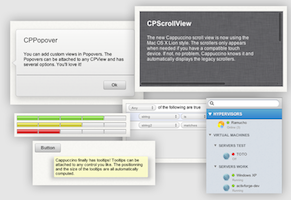
\includegraphics{figures/cappuccino-widgets.png}
\caption{Un ejemplo de los diferentes controles que vienen incluidos en
Cappuccino. Puede apreciarse el diseño estilo OS X que trae.
\label{figure:cappuccino}}
\end{figure}

Una de las características interesantes de este framework (aunque no es
la que más se publicita), es la capacidad de usar el constructor de
interfaces de \href{https://developer.apple.com/xcode/}{Xcode} {[}6{]}
--- Interface Builder --- para crear las interfaces. Eso sí, no todos
los componentes que están disponibles en Xcode están implementados en
Cappuccino, y agregar elementos inexistentes no siempre arroja errores
fáciles de descubrir. Además, desarrollar usando esta técnica, requiere
instalar varios componentes (entre ellos, Xcode, que no es liviano) y se
necesita un computador Mac, dado que Xcode no funciona en otras
plataformas. Por si eso no fuera poco, el ir y venir entre Xcode y el
editor que se use para Cappuccino hace que la experiencia sea todo menos
placentera para el desarrollador.

Además de lo anterior, tiene otras desventajas. Por un lado, es
necesario aprender un lenguaje nuevo (Objective-J) y utilizar un
framework completamente distinto a todos los conocidos (casi todos están
programados en Javascript directamente). Por otro lado, hay varios
controles esenciales que no están implementados, como por ejemplo, un
control de entrada de texto multilínea no está soportado actualmente por
el framework (aunque existen herramientas de terceros).

\subsubsection{Ext JS}

\href{http://www.sencha.com/products/extjs/}{Ext JS} {[}7{]} es un
framework con bastante tiempo en el mercado. Tiene soporte para una gran
variedad de componentes y es muy poderoso. Una de las ventajas
importantes de este framework, es que existe una empresa bastante
importante detrás: \href{http://www.sencha.com/}{Sencha Inc}. Esto
asegura que el framework tiene soporte detrás, y que existe mucha gente
preocupada constantemente de su desarrollo. Incluso, esta empresa ofrece
soporte técnico pagado para este framework.

Este es un framework bastante poderoso, a la par e incluso por sobre
Cappucino y otros similares. Al llevar bastante tiempo circulando (desde
el 2007 {[}8{]}), es un framework con una gran cantidad de componentes y
características disponibles que lo hacen muy poderoso. Se diferencia en
casi las mismas cosas con Backbone que Cappuccino, al tener integrados
muchísimos componentes como botones, tablas, ventanas, entre otros, pero
con la diferencia de que este framework sí está escrito en Javascript
directamente, por lo que no hace falta aprender un lenguaje nuevo.

Ahora bien, tiene sus desventajas. Es un framework muy completo y
dominarlo toma más tiempo que otros. No es un framework fácil de usar y
no existe una gran comunidad detrás (no existen muchos sitios
desarrollados con esta plataforma, al menos no sitios públicos), por lo
que encontrar tutoriales e información al respecto no es tarea fácil.
Además, una de las mayores desventajas, es que este framework no es
gratuito para desarrollo comercial. Si se desea desarrollar una
aplicación web y mantener el código propietario, se deben cancelar (por
lo bajo) \$329 dólares americanos {[}9{]}, valor a veces prohibitivo
considerando que la mayoría de los otros frameworks son gratuitos.

\subsection{Herramientas Actuales}

Ahora que se han visto una variedad de frameworks disponibles para
desarrollar aplicaciones web, se procederá a analizar el mundo de las
herramientas para el desarrollo de éstas. El enfoque de esta sección es
analizar diferentes programas y servicios que se ofrecen, que son en
alguna forma similares a lo que se quiere lograr con Switch IDE.

\subsubsection{Sencha Architect}

Si se tuviera que elegir una herramienta para describir lo que se quiere
lograr con Switch, sería
\href{http://www.sencha.com/products/architect}{Sencha Architect}
{[}10{]}. Sencha Architect es una herramienta de los mismos creadores
del framework Ext JS, y es lo que más se asemeja a lo que se quiere
lograr con esta memoria. Es bastante poderosa, y permite desarrollar
aplicaciones web y móviles (basadas en web, no nativas) de manera
visual, de una forma bastante similar a lo que se quiere lograr con
Switch IDE.

\begin{figure}[htbp]
\centering
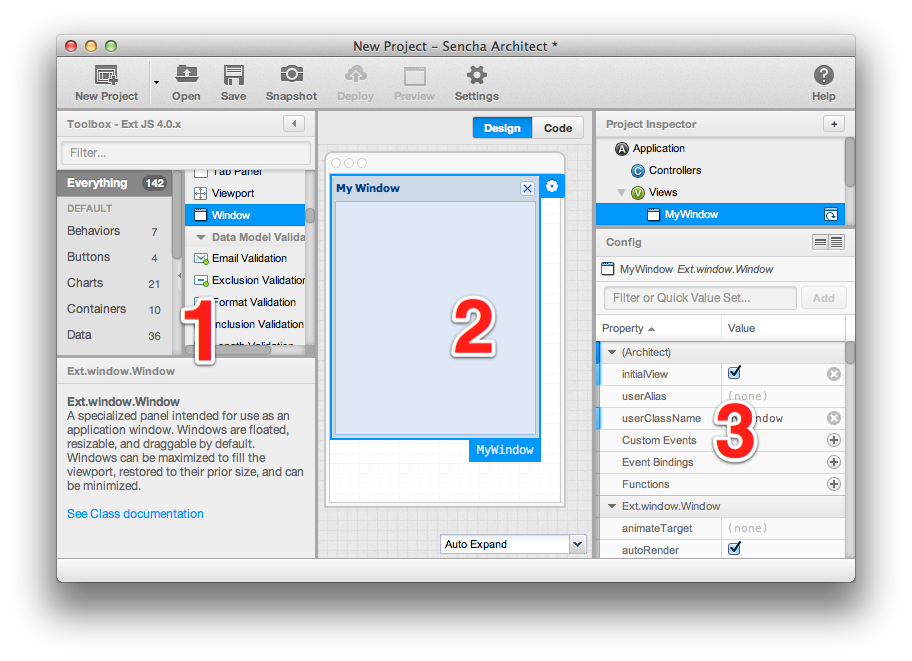
\includegraphics{figures/sencha-architect-big.png}
\caption{Sencha Architect: La ventana de trabajo
\label{figure:sencha-architect}}
\end{figure}

Sencha Architect es la herramienta que más se asemeja a un IDE para
desarrollo de aplicaciones nativas (como Xcode o Microsoft Visual
Studio). Posee una barra lateral con componentes (ver Figura
\ref{figure:sencha-architect}, el número 1), un área central de trabajo
(número 2) y propiedades de los diferentes componentes que existan en el
área de trabajo (número 3).

Las ventajas de esta herramienta son claras: es posible crear las vistas
de las aplicaciones directamente, arrastrando componentes. De la misma
forma que herramientas para desarrollo nativo, esto ahorra tiempo al
momento de desarrollar.

Las desventajas son varias, eso sí. Por un lado, el desarrollador está
obligado a trabajar con Ext JS como framework (que, como ya se dijo
antes, no es fácil de aprender y usar), y por otro lado, la licencia de
uso de este software no deja de ser considerable: \$399 dólares
americanos {[}11{]} al momento de escribir este documento. Esto es un
monto realmente alto, pues si se compara esto con el precio de un editor
de código relativamente bueno (como lo son TextMate o Sublime Text 2,
ambos cercanos a los \$50 dólares), es una inversión de consideración.
Además, a ese valor hay que agregarle otros \$329 por la licencia de uso
de Ext JS {[}9{]}, si es que se quiere para uso comercial.

\subsubsection{Divshot}

\href{http://divshot.com/}{Divshot} {[}12{]} es una de las herramientas
que inspiró la presente memoria. Es una aplicación de prototipado rápido
basado en web. Fue creada en abril de 2012, por lo que es una
herramienta relativamente nueva y, de hecho, no está abierta al público
aún. Se logró conseguir una licencia de uso en esta fase para poder
estudiar el poder de esta herramienta, y se llegó a la conclusión de que
realmente tiene mucho potencial.

Permite, utilizando Twitter Bootstrap {[}13{]}, crear prototipos de
sitios y aplicaciones web arrastrando componentes, de la misma forma que
IDEs como Xcode o Microsoft Visual Studio. En la presente memoria, se
quiere lograr un comportamiento muy parecido para la creación de vistas,
por lo que se podría considerar que Divshot es una de las inspiraciones
más grandes para esta memoria.

Entre las ventajas que presenta la herramienta, está la facilidad con la
que se pueden crear prototipos de vistas. Sólo arrastrando componentes,
se puede llegar a una vista en pocos minutos. Además, es posible
previsualizar los resultados fácilmente, e incluso exportar a
HTML\footnote{\textbf{Hypertext Markup Language:} es el lenguaje de
  etiquetas utilizado para las páginas web. Todas ellas están hechas con
  esto, más una combinación de otros lenguajes. {[}14{]}} con un sólo
click. Lo mejor de todo, es que el HTML generado está muy bien ordenado
y formateado.

Desventajas no tiene muchas. Es una herramienta muy puntual y bien
diseñada, y, como aún está en fases de desarrollo, en constante mejora.
Ahora bien, no es un ``competidor'' directo de Switch IDE, dado que no
es una herramienta para programar. Simplemente permite crear vistas, que
es sólo un componente de Switch.

\begin{figure}[htbp]
\centering
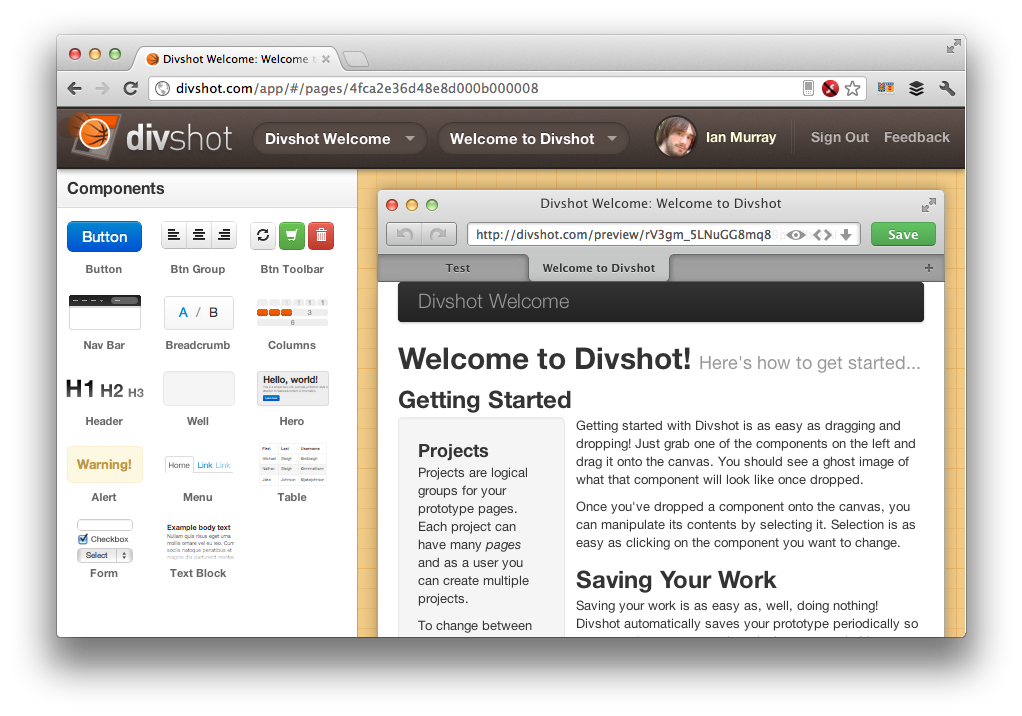
\includegraphics{figures/divshot-big.png}
\caption{La ventana principal de Divshot. Se pueden apreciar los
componentes en la barra lateral izquierda, con la vista a la derecha,
donde se arrojan los componentes. \label{figures:divshot}}
\end{figure}

\subsubsection{eXo Cloud IDE}

\href{http://cloud-ide.com}{eXo Cloud IDE} {[}15{]} es un entorno de
desarrollo integrado, en la nube. Tiene varias características que lo
hacen una buena opción al momento de querer colaborar o mantener el
código alojado en internet. Soporta una gran variedad de lenguajes
(entre ellos Java, Ruby y Python) y frameworks (como Ruby on Rails,
Spring o incluso Google App Engine).

Además de lo anterior, soporta plataformas como Heroku para subir
cambios a servidores directo desde el navegador, e incluso tiene soporte
para versionamiento con Git {[}16{]}.

Como cualquier IDE nativa estilo Xcode o Microsoft Visual Studio, tiene
un visor de los archivos actualmente abiertos (ver Figura
\ref{figure:exo-ide}, número 1) y el editor de código mismo (número 2).

\begin{figure}[htbp]
\centering
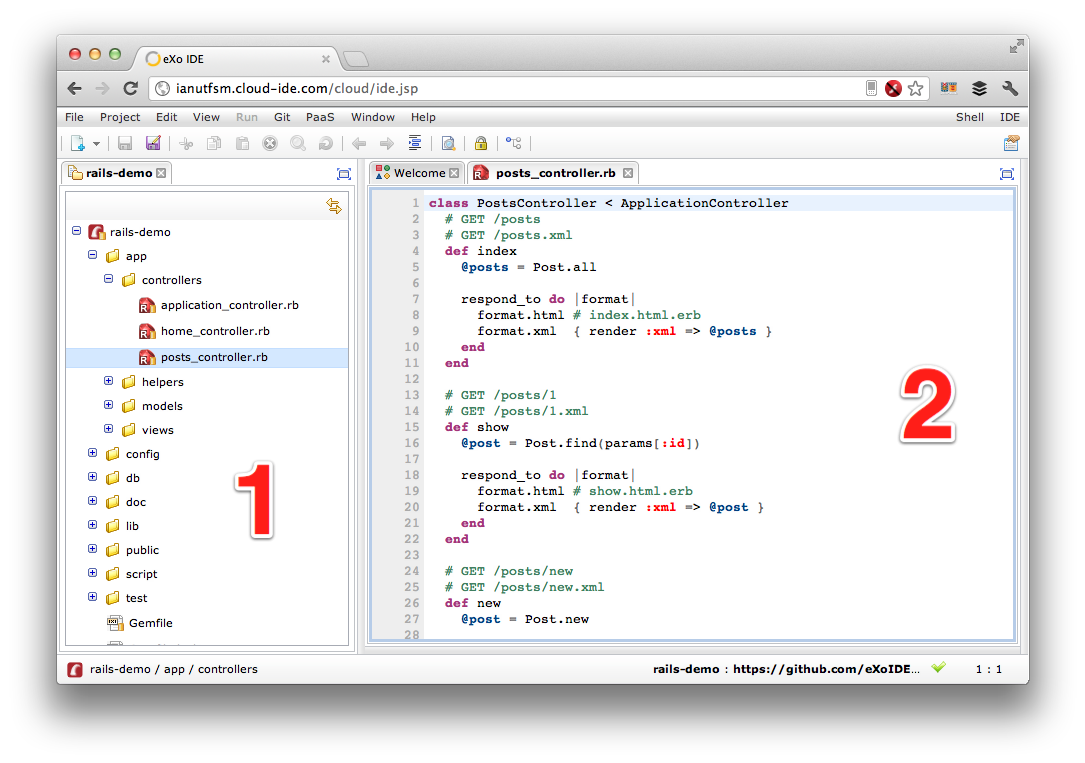
\includegraphics{figures/exo-ide-big.png}
\caption{eXo Cloud IDE: un entorno de desarrollo integrado, en la
nube\label{figure:exo-ide}}
\end{figure}

Las ventajas que provee esta herramienta son el no tener que depender de
un sólo equipo para desarrollar. Al mantener el código en la nube, sólo
es necesario conectarse al sitio web y empezar a trabajar. Por esto
último, tampoco es necesario instalar las diferentes herramientas
necesarias para desarrollar (como puede ser instalar Ruby o Python, que
a veces es engorroso).

Ahora bien, tiene sus desventajas, siendo la más importante el hecho de
que no permite desarrollar vistas de forma visual (que es lo que uno
espera de una herramienta integrada de este estilo). Además, al no estar
enfocado en un framework de desarrollo específico, no es muy poderoso al
momento de elegir alguno (en términos de autocompletado de código por
ejemplo). Relacionado con esto último, no permite desarrollar
aplicaciones de lado de cliente, sólo de lado de servidor, por lo que
también está limitado por ese lado. Además, desarrollar aplicaciones con
los frameworks que soporta por lo general implica utilizar mucho el
terminal de comandos para realizar pruebas, y en un ambiente web, eso no
es fácilmente replicable.

\subsubsection{Wavemaker}

\href{http://www.wavemaker.com/}{Wavemaker} {[}17{]} es una herramienta
que permite generar ``bases de datos'' de manera visual. El objetivo
principal de esta aplicación es poder crear sistemas de manejo de datos
de manera fácil, escribiendo la menor cantidad de código posible.

Esta herramienta se asemeja más a lo que es Microsoft Access. La idea es
poder crear interfaces para guardar y organizar información rápidamente
y sin programar. Es una aplicación enfocada más a gente que no tiene
conocimientos de programación, aunque según los creadores de Wavemaker,
las aplicaciones que se generan son aplicaciones Java completas, que
pueden ser extendidas más adelante programando Java directamente.

Las ventajas dependen realmente de lo que se quiera hacer con la
herramienta. Si el usuario no tiene conocimientos en el área de
desarrollo de software, entonces la herramienta es bastante útil, aunque
los resultados no son muy complejos. Por otro lado, si se le mira desde
el punto de vista de un desarrollador, la herramienta no ofrece mayores
beneficios a las anteriormente mencionadas.

\subsubsection{Zoho Creator}

\href{http://www.zoho.com/creator/}{Zoho Creator} {[}18{]} es un
servicio web que tiene más o menos el mismo enfoque que Wavemaker: crear
bases de datos simples sin programar. Ahora bien, se diferencia un poco
con Wavemaker en el sentido de que es un servicio, pagado, que permite
crear aplicaciones en la nube y mantenerlas ahí, mientras que la
herramienta anterior permite crearlas y exportarlas, para luego incluso
extenderlas si es que se tienen conocimientos.

Si bien Zoho Creator es una herramienta relativamente poderosa y fácil
de usar, no es una herramienta que utilizaría un desarrollador. Hay
varias razones para esto último. Primero, no permite exportar lo creado
para alojarlo en otro servidor; segundo, no es una herramienta de
desarrollo que permita crear aplicaciones de lado de cliente o de
servidor, sino que permite crear simples bases de datos; y tercero, no
es una herramienta gratuita o de código abierto, lo que hace que lo
creado con ella tenga ciertas limitaciones en cuanto a licencias.

\clearpage
\newpage

\section{Propuesta de Solución}

Para solucionar el problema identificado, se propone una herramienta
web, basada en \emph{Backbone} y \emph{Ruby}, que permita editar una
aplicación web completa en el mismo navegador. Sus principales
características serían:

\begin{itemize}
\item
  Dar una estructura a las aplicaciones que se desarrollen con Backbone
\item
  Facilitar la creación de vistas mediante un editor que permita
  arrastrar los diferentes componentes y ahorrar el tiempo gastado en
  ello
\item
  Implementar atajos de teclado de manera similar a cómo lo haría una
  IDE de escritorio
\item
  Permitir ensamblar y probar la aplicación de manera similar a cómo lo
  haría un programa nativo
\end{itemize}

La herramienta no puede funcionar sólo de lado de cliente
(exclusivamente en el navegador), dado que algunas funciones deben ser
ejecutadas en el servidor, como por ejemplo la compilación de los
archivos Javascript y levantar una instancia de un servidor para probar
lo que el usuario esté desarrollando. Por esto, es necesario implementar
este proyecto en dos partes distintas, pero dependientes.

Por un lado, se tiene el servidor, que tendrá la tarea de manipular los
archivos de cada proyecto que el usuario cree y desarrolle. Además,
tendrá la tarea de ejecutar ciertos comandos necesarios para la creación
y prueba de los proyectos, que simplemente no es posible ejecutar en el
navegador. El hecho de que exista un ``backend'' (como se le llamará de
ahora en adelante), permite además dar lugar a futuras características
imposibles de llevar a cabo de otra forma, como por ejemplo soporte para
repositorios Git, que deben ser manejados en el servidor exclusivamente.

Por otro lado, está el cliente. El cliente es básicamente el
``frontend'' (como se le llamará de ahora en adelante). Es la interfaz
gráfica y es lo que interactúa con el usuario, en el navegador. La mayor
parte del trabajo recaerá en esta parte, dado que es lo que el usuario
ve y utiliza para trabajar. Además, es la parte del proyecto que
contendrá el editor de vistas, lo que requerirá un esfuerzo no mínimo
para funcionar.

\subsection{Elección de Herramientas para el Backend}

Para desarrollar el backend se escogió el lenguaje de programación
\emph{Ruby}. Las razones para la elección de este lenguaje son varias:
la familiaridad que tiene el autor con éste; su simplicidad para
desarrollar tareas relativamente complejas en otros lenguajes; la
infinidad de librerías disponibles para facilitar diferentes tareas
(como por ejemplo \emph{Grit}, una librería para manejar repositorios
Git directo desde Ruby)\footnote{Cita?}.

Para desarrollar el backend no se utilizará Ruby puro. Lo que se quiere
desarrollar en el lado del backend es básicamente una API (Application
Programming Interface), que el frontend utilizará parar funcionar
correctamente. Existen varias formas de programar APIs en Ruby, donde
las más populares son Ruby on Rails y Sinatra.

La primera --- Ruby on Rails --- ha comenzado a ser muy popular en estos
últimos años por ser un framework extremadamente completo. Facilita
enormemente una infinidad de tareas que lo hacen una herramienta ideal
para todo tipo de proyectos web. Sin embargo, al ser una herramienta tan
completa, agrega bastante \emph{overhead}. Además, es una herramienta
ideal para crear proyectos grandes y muy complejos, y dado que el
backend de el presente trabajo no requerirá tanta complejidad, se
convierte en una alternativa no tan ideal para este trabajo.

La segunda --- Sinatra --- podría considerarse el hermano menor de Ruby
on Rails. Es un framework muchísimo más simple, y, por ende, mucho más
liviano. Inicia más rápido y, en general, se desempeña mejor que su
contraparte. Tiene la desventaja de no poseer tantas facilidades para
desarrollar sitios complejos y grandes, pero dado que el backend de este
proyecto no requerirá tanto trabajo, es la opción ideal.

El backend requerirá una base de datos para poder guardar información de
los usuarios y proyectos. Se pensó en dos alternativas: MySQL y MongoDB.
La primera es una base de datos convencional, poderosa y muy popular. La
segunda es una base de datos de la familia conocida como ``NoSQL'', es
decir, no es una base de datos tradicional. Permite almacenar
``documentos'', o, más específicamente, objetos del estilo JSON. Además,
no acepta consultas SQL, si no que las consultas se realizan utilizando
métodos directamente en la base de datos.

Las ventajas que tiene MongoDB sobre MySQL son varias. Por un lado, es
un sistema de bases de datos rápido y liviano, soporta escalamiento
horizontal fácilmente, e incluso permite almacenar archivos en él usando
una tecnología llamada GridFS\footnote{Http://www.mongodb.org/display/DOCS/GridFS.}.

En términos de uso, existen librerías en Ruby para interactuar con ambas
bases de datos. Para MySQL, es posible usar ActiveRecord\footnote{Link!},
un ORM\footnote{Object Relational Mapper.} muy popular y muy poderoso
que permite hacer consultas a la base de datos sin utilizar SQL. Para
MongoDB, existe Mongoid\footnote{Link!}, un ODM\footnote{Object Document
  Mapper.} que provee una interfaz muy similar a ActiveRecord.

Dadas las ventajas que provee MongoDB y la posibilidad de utilizar un
ODM muy similar a ActiveRecord, se decidió utilizar MongoDB.
Afortunadamente, en caso de querer cambiar el sistema de base de datos,
no se requerirían muchos cambios dadas las similitudes de las librerías
utilizadas.

\subsection{Elección de Herramientas para el Frontend}

Dado que la solución que se propone es una herramienta para desarrollar
aplicaciones en Backbone utilizando Twitter Bootstrap, lo lógico es
desarrollar esta solución usando las mismas herramientas. Se escogió
Backbone dada su alta popularidad. Esto asegura que el framework es
bastante sólido y que existen variadas librerías y herramientas estables
para él. Por otro lado, si bien Backbone es un framework poderoso, es
bien simple, lo que da más libertad sobre como afrontar diferentes
problemas.

Ahora, Backbone es un framework que no da una estructura a las
aplicaciones que se desarrollan con él. A diferencia de Ruby on Rails,
por ejemplo, la tarea de estructurar la aplicacion en carpetas o módulos
depende completamente del desarrollador. En este punto se asemeja mucho
más a Sinatra que a Ruby on Rails. Esto puede considerarse una
desventaja, dado que sistemas complejos tienden a crecer y desordenarse
bastanta si no se aplica una estructura desde un principio. Por esto, es
que se decidió utilizar Brunch\footnote{Poner referencia a esto!}.
Brunch es un ensamblador de aplicaciones (``application assembler'' en
inglés). Básicamente, basándose en un esqueleto, organiza aplicaciones
en carpetas. Soporta diferentes frameworks y lenguajes, desde Backbone a
Knockout\footnote{Referencia!}, usando Javascript o
Coffeescript\footnote{Referencia.}. Además de entregar una estructura,
las ensambla, es decir, toma todos los archivos y los junta en uno sólo
de manera de optimizar la aplicación cuando esté en producción. Es más,
incluye un servidor web de desarrollo, que detecta cambios en los
archivos y reensambla todo el sitio de manera de poder hacer pruebas más
rápida y fácilmente.

En lo que respecta la decisión de lenguaje de programación, no hay
muchas alternativas. Es posible desarrollar la solución usando
Javascript o Coffeescript. Existen otras alternativas, pero al momento
de escribir este documento no se encuentran en etapas estables de
desarrollo ni madurez. Javascript es un lenguaje poderoso pero a la vez
de relativo bajo nivel. Ciertas cosas son un tanto tediosas de
programar, como recorrer arreglos por ejemplo. En cambio, Coffeescript,
un lenguaje de programación escrito por Jeremy Ashkenas que apareció en
el 2009\footnote{Https://github.com/jashkenas/coffee-script/commit/8e9d637985d2dc9b44922076ad54ffef7fa8e9c2.}
que compila a Javascript, hace que desarrollar en Javascript sea mucho
más cómodo y simple, sin perder desempeño ni funcionalidad (pues compila
directamente a Javascript). Además, hace muchísimo más fácil programar
``orientado a objetos''. Si bien ECMAScript (la base de Javascript) está
definido como orientado a objetos,\footnote{Http://www.ecma-international.org/publications/files/ECMA-ST/Ecma-262.pdf
  página 1.} su estilo es diferente al resto de los lenguajes.
Coffeescript agrega palabras clave como \texttt{class} y
\texttt{extends} de manera de facilitar escribir clases y manipular
objetos en este lenguaje.

Por último, para el diseño y estructura de la interfaz, se decidió
utilizar \emph{Twitter Bootstrap}. Bootstrap es un conjunto de
componentes y un sistema de estructurado para páginas web, que hace la
tarea de crear y diseñar un sitio muy simple. Trae consigo una enorme
cantidad de componentes (botones, barras de progreso, etc.), además de
facilitar el diseño de formularios y componentes similares muy comunes
al momento de crear aplicaciones web. No sólo se utilizará Twitter
Bootstrap para crear el frontend, sino que también se utilizará para el
diseñador de interfaces, dado que tiene todas las ventajas descritas
anteriormente.

\clearpage
\newpage

\section{Construcción de la Solución}

Este capítulo tiene por objetivo detallar todo el proceso del diseño y
desarrollo de la solución propuesta anteriormente. Se dividirá en los
siguientes subcapítulos:

\begin{enumerate}[a.]
\item
  Diseño de la solución: básicamente se explicará cómo ambas componentes
  (frontend y backend) interactuarán entre sí. Además, cómo funcionarán
  ambas partes en términos de manipulación de archivos y el proyecto
  completo. Por último, se explicará cómo se diseñó el componente
  principal de la solución (el editor de interfaces).
\item
  Primera etapa de construcción: el desarrollo de la solución se dividió
  en dos etapas principalmente. Primero, se desarrolló lo que se
  denominó una ``base'' del programa. Esta etapa contempló el desarrollo
  de gran parte del backend y, en el frontend, una herramienta que
  permitiera crear proyectos nuevos, crear, editar y eliminar archivos,
  compilar y correr el proyecto.
\item
  Segunda etapa de construcción: la segunda parte del desarrollo se
  enfocó en desarrollar y perfeccionar el editor de interfaces. Dado que
  este componente es el grueso de la solución, se decidió dedicar una
  etapa completa a él.
\end{enumerate}

\subsection{Diseño de la Solución}

\subsubsection{Backend}

La solución es una aplicación mayoritariamente de lado de cliente, por
lo que la mayor cantidad de lógica debe ir en este lado. Por esta razón,
se diseñó el servidor de la forma más simple posible. Las tareas
principales que tiene el servidor o backend de la aplicación son:

\begin{itemize}
\item
  Autentificar usuarios
\item
  Generar proyectos utilizando Brunch
\item
  Manipular los archivos. Esto incluye crear, eliminar, renombrar y
  actualizar archivos (o sea, recibir el contenido de ellos y guardarlo
  a disco)
\item
  Ensamblar el proyecto
\item
  Levantar un servidor estático que permita al usuario probar su
  proyecto
\end{itemize}

Algunas de estas tareas son realizadas por la utilidad Brunch, por lo
que sólo es necesario hacer que el servidor ejecute un comando en la
consola para llevarlas a cabo. El resto de las tareas son básicamente
manipulación de archivos, para lo cual cualquier lenguaje de
programación trae funciones o librerías (y Ruby no es ninguna
excepción).

Se decidió utilizar una aproximación a lo que es REST\footnote{Explicar
  esto.} para los servicios que proveerá el backend. En REST, la idea es
representar objetos, y exponer diferentes métodos para tales objetos. En
este caso, se decidió que deben existir 3 objetos diferentes: usuarios,
proyectos y archivos.

\begin{itemize}
\item
  Usuarios: dado que la idea es que varios usuarios puedan utilizar el
  sistema a la vez, debe existir esta entidad en el servidor (y por ende
  en la base de datos).
\item
  Proyectos: es casi la base de todo. Cada proyecto contendrá los
  diferentes archivos y carpetas, y pertenecerá a un usuario.
\item
  Archivos: esto se refiere a archivos y carpetas. Por la forma en la
  que se manipulan los archivos en el servidor y en el cliente, es más
  conveniente manejarlos de (casi) la misma forma. Esto último se
  refiere a la forma en la que se obtienen los archivos en el servidor,
  y las acciones que se realizan en ellos. Ambos archivos y carpetas se
  crean y eliminan, como también se renombran. La única diferencia
  substancial es que las carpetas no tienen contenido y no se actualizan
  como el resto de los archivos.
\end{itemize}

El servidor autentificará a los usuarios utilizando sus cuentas de
GitHub y OAuth. OAuth es un protocolo de autentificación y autorización
que permite al usuario registrarse e ingresar a la aplicación con un
sólo click (dos si ingresa por primera vez). Dado que esta es una
herramienta enfocada a programadores, y considerando que GitHub es una
plataforma conocida por cualquier desarrollador que se mantenga al día,
utilizar este sistema para autentificar a los usuarios es simple y
conveniente. Por el lado de servidor, basta con incluir una librería que
redirige a los usuarios a las URLs específicas y crear un registro en la
base de datos si es que el usuario está ingresando por primera vez.

\subsubsection{Frontend}

El frontend tendrá dos tareas principalmente. Primero, deberá permitir a
los usuarios autentificarse. Para esto, y para efectos del presente
trabajo, será una simple página web que redirija al usuario a GitHub
para autentificarse usando este sistema. Segundo, deberá proveer al
usuario con la IDE que se quiere construir en este documento.

\textbf{\emph{EXPLICAR DE QUÉ TRATA LA PÁGINA DE AUTENTIFICACIÓN A
GRANDES RASGOS, SCREENSHOTS Y TODO}}

La IDE misma se dividirá en tres componentes principales: la barra
lateral izquierda para explorar los archivos del proyecto, la barra
lateral derecha con componentes visuales (como botones, formularios,
etc.), y la sección central que contendrá el código del archivo
actualmente seleccionado o la vista previa en caso de estar editando una
vista.

Contará además con una barra superior con un menú (al igual que
cualquier aplicación de escritorio), pero dado que proveerá simples
accesos directos a funciones que se explicarán más adelante no se
detallará su diseño ni implementación.

\paragraph{Definición de Objetos}

\label{section:object-definition}

En esta sección se pretende explicar qué objetos existirán en el
frontend, sus responsabilidades y cómo interactuarán entre ellos.
Primero se definirán algunos conceptos necesarios para entender de qué
tipos de objetos se estará hablando.

\begin{description}
\item[Modelo]
Representa un objeto en un proyecto, como por ejemplo un archivo, una
carpeta o el proyecto mismo. Cada modelo es responsable de persistir su
estado de alguna forma (comunicándose con un servidor o almacenando
datos en el mismo navegador).
\item[Colección]
Es básicamente una lista de instancias de un tipo de modelo. Por
ejemplo, una carpeta podría considerarse una colección de archivos
(siendo cada archivo una instancia de un modelo).
\item[Vista]
Una vista en Backbone es un archivo que se encarga de presentar
información al usuario, y además de interactuar con él, por ejemplo
ejecutando funciones cuando se haga un click en un botón. Una vista por
lo general presenta un modelo (o una colección). Por ejemplo, se puede
tener una vista para cada instancia de un archivo, o bien se pueden
tener vistas que no presenten a ningún modelo en particular.
\item[Template]
Un template es un trozo de HTML que una vista utiliza para generar lo
que el usuario ve. Si bien no son enteramente necesarias y una vista
podría generar todo lo que necesita con Javascript, hacen la tarea algo
más fácil. Contrario a lo que pueda suponerse, el editor visual en el
que se trabajará en este documento editará los templates, y no las
vistas.
\end{description}

\subparagraph{Modelos y Colecciones}

A continuación se explicará a grandes rasgos los modelos y colecciones
que existirán en el frontend. Se tendrán modelos para los proyectos y
los archivos. Cada uno se encargará de comunicarse con el backend para
obtener los datos que le sean necesarios o bien para guardar los
cambios.

\begin{description}
\item[El modelo de proyecto]
Guardará el nombre de éste y una referencia a una colección de los
archivos que se encuentren en la raíz de su carpeta. Tendrá como
responsabilidades crear archivos y carpetas, ensamblar el proyecto e
iniciar el servidor de pruebas. Estas acciones se complementan con
llamadas al backend que realizan las tareas mismas.
\item[El modelo de archivo]
Se encargará de guardar el nombre y el contenido (en caso de que
corresponda) del archivo o carpeta al que representa, además de guardar
una referencia al proyecto al que pertenece y . Tendrá como
responabilidades pedir su contenido, actualizarlo, renombrar y eliminar
el archivo del sistema. Todas estas acciones se complementan además con
llamadas al backend.
\item[La colección de archivos]
Tendrá como responsabilidad ordenar las listas de archivos una vez que
la haya obtenido (además de guardar una referencia a cada modelo de
archivo que le corresponda). Ordenar las listas de archios es importante
pues el backend arroja una lista de archivos ordenada alfabéticamente,
pero, dado que archivos y directorios son considerados de la misma forma
en el backend, es necesario ordenar la lista de manera que los
directorios queden arriba. Esto facilita encontrar archivos para el
usuario.
\end{description}

\subparagraph{Vistas}

Cada una de las siguientes vistas considera un template asociado.

\begin{description}
\item[Explorador de Archivos]
se colocará en la barra lateral izquierda, y tendrá dos listas de
archivos. Una lista de archivos actualmente abiertos y la lista de
archivos y directorios en el proyecto. Tendrá entre sus
responsabilidades mantener una lista de archivos que se encuentran
actualmente abiertos para que el usuario pueda navegar entre ellos.
\item[Archivo]
Esta vista representará a un archivo en la vista anterior (exporador de
archivos). Mostrará su nombre y un icono que represente si es un
directorio, un archivo o una vista editable con el editor que se
construirá. Entre sus responsabilidades están abrir los archivos (o sea,
abrir el archivo en el editor de código o en el editor de vistas en caso
que corresponda), embeber listas de archivos en caso de que se clickee
un directorio y permitir al usuario renombrar archivos, mostrando un
menú contextual.
\item[Editor de Texto]
Esta vista contendrá el editor de archivos de texto (editor de código).
Sus responsabilidades serán mostrar un editor con resaltado de sintaxis
y modificar el modelo de archivo que corresponda para guardar cambios.
\item[Editor de Vistas]
esta vista mostrará templates y, en una barra lateral derecha,
diferentes componentes para que el usuario los arrastre y agregue.
Contará además con un editor de código HTML, en caso de que el usuario
quiera editar la vista o realizar cambios que el editor no permita
directamente. Tiene las mismas responsabilidades que el editor de texto.
\end{description}

\paragraph{Diseño del Editor de Templates}

El editor de interfaces se construirá de manera que el usuario pueda
arrastar componentes como botones o campos de texto directamente en una
vista previa del template que esté editando. El contenido de los
archivos de templates es simplemente HTML, por lo que es posible
presentarlos directamente en la aplicación. Este contenedor o vista
previa del template se le llamará ``canvas'' de ahora en adelante.

El objetivo es que el usuario arrastre elementos hacia el canvas de la
misma forma en la que se hace en Xcode o Visual Studio. El sistema debe
proveerle retroalimentación visual mostrando el objeto que está
arrastrando y además mostrar en qué lugar quedararía el elemento una vez
que el usuario lo suelte.

Para implementar este concepto de arrastrar y soltar, se utilizará
jQuery UI. esta librería provee, entre otras cosas, métodos para
habilitar el arrastrado de elementos en una página. El usuario
arrastrará un elemento, y, mediante las llamadas de jQuery, se colocará
el elemento en donde el usuario tenga su cursor en el momento, a manera
de proveer retroalimentación visual. En cuanto el usuario suelte el
elemento, se agregará su correspondiente fragmento de HTML en el
template, lo que se reflejará en el canvas en tiempo real.

\begin{figure}[htbp]
\centering
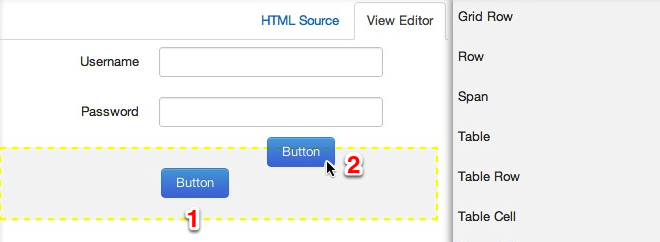
\includegraphics{figures/drag-editor.png}
\caption{Los diferentes elementos de retroalimentación visual que se
presentan al arrastrar un componente. \label{figures:drag-editor}}
\end{figure}

En la Figura \ref{figures:drag-editor} se pueden apreciar los diferentes
elementos de retroalimentación al momento de arrastrar un elemento. En
el punto 1 se pueden apreciar, primero, un borde amarillo al rededor del
elemento en donde ``caería'' el componente. Además, en el mismo número,
puede visualizarse cómo se vería el componente (en este caso un botón)
una vez que el usuario lo deje ahí. En el número 2, puede verse el mismo
componente, que sigue al cursor mientras el usuario esté arrastrando.
Esto le muestra al usuario qué es lo que está arrastrando.

De esta forma, el desarrollador puede ver, por un lado, qué componente
estaría agregando al canvas y, por otro lado, cómo quedaría éste una vez
que lo agregue.

\subsection{Primera Etapa de Construcción}

\subsubsection{Creación del Entorno de Trabajo}

En esta sección se detallarán cómo se crearon y estructuraron los dos
entornos de trabajo, tanto para el backend como para el frontend.

Ambos entornos de trabajo se crearon en carpetas independientes (dada su
naturaleza) y se inicializaron repositorios Git en cada una, a manera de
mantener un control de versiones en cada una.

Para el control de versiones no se utilizó ninguna estrategia en
especial. Dado que sólo el autor estará desarrollando, no valdría la
pena implementar alguna estrategia de ramas o algo parecido para el
control de versiones. Simplemente se utilizó la rama principal
(\texttt{master} en Git), y se fueron creando ``commits'' cuando se
considerara necesario.

\paragraph{Entorno de Trabajo para el Backend}

El backend utilizará Ruby con Sinatra. Sinatra se diferencia de, por
ejemplo, Rails, en que es un framework mucho más simple. Por esto, es
que no posee utilidades para crear directorios de trabajo. La idea
detrás de Sinatra es crear todo en un sólo archivo. Si bien esto es
posible, e incluso aconsejable para algunas aplicaciones, no lo es para
ésta, en donde se tendrán diferentes modelos y controladores. Por lo
tanto se definió la siguiente estructura para el backend:

\begin{itemize}
\item
  \texttt{api}

  \begin{itemize}
  \item
    \texttt{v1}

    \begin{itemize}
    \item
      \texttt{config}: contiene diferentes archivos de configuración
    \item
      \texttt{controllers}: los diferentes controladores
    \item
      \texttt{models}: los modelos de usuario y proyecto
    \item
      \texttt{app.rb}: este archivo es la base de la aplicación Sinatra,
      pues nicializa ciertas configuraciones y contiene métodos
      compartidos por los controladores
    \item
      \texttt{boot.rb}: este archivo es cargado inicialmente y se
      encarga de incluir las diferentes librerías y archivos para
      incializar el servidor
    \end{itemize}
  \end{itemize}
\item
  \texttt{projects}: será el contenedor de los diferentes proyectos que
  crearán los usuarios
\item
  \texttt{public}: esta carpeta sirve archivos estáticos directamente,
  como imágenes
\item
  \texttt{Gemfile}: archivo utilizado por Bundler (una librería de Ruby)
  para definir qué librerías y en qué versiones utilizará el backend
\item
  \texttt{config.ru}: archivo utilizado para levantar el servidor
\end{itemize}

Se decidió estructurar el backend en carpetas de versiones. La idea
detrás de esto es poder dividir cada versión de la API de manera de no
perder compatibilidad con posibles clientes que estén basados en una
versión de la API. Por ejemplo, de llegar a crearse un cliente para
tablets, cada cliente estaría atado a una versión específica. Si se
cambiara algún método (o se descontinuara), el cliente automáticamente
fallaría. En cambio, teniendo diferentes versiones, se puede mantener
esta compatibilidad.

Se creó además una carpeta llamada \texttt{projects}. Esta carpeta (que
no es accesible directamente), guarda cada uno de los proyectos de cada
usuario. Cada vez que se inicialice uno nuevo, se creará una subcarpeta
en este directorio con la estructura determinada.

El archivo \texttt{Gemfile} es un archivo que utiliza la librería
Bundler\footnote{Citar blablabla.}. Esta utilidad permite especificar
librerías externas que se quieren incluir en un proyecto (en este caso
el backend) y especificar sus versiones. Por ejemplo, un extracto de un
archivo Gemfile podría verse así:

\begin{Shaded}
\begin{Highlighting}[]
\NormalTok{gem }\StringTok{'sinatra'}\NormalTok{, }\StringTok{'1.3.3'} \CommentTok{# Especifica que se utilizará la versión 1.3.3}

\NormalTok{gem }\StringTok{'activerecord'}\NormalTok{, }\StringTok{'~> 3.2'} \CommentTok{# Especifica que se utilizarán }
                             \CommentTok{# versiones 3.2.X}

\NormalTok{gem }\StringTok{'haml'} \CommentTok{# Especifica que se utilizará la última versión}
\end{Highlighting}
\end{Shaded}

La gran utilidad de esta herramienta es que, al momento de ejecutar en
la consola \texttt{bundle install}, las versiones especificadas son
descargadas y se crea un archivo llamado \texttt{Gemfile.lock} que
guarda las versiones que están siendo utilizadas. De esta forma, cuando
otro desarrollador descargue el repositorio y ejecute nuevamente
\texttt{bundle install} para instalar las dependencias, se descargarán
exactamente esas versiones y ambos desarrolladores tendrán el mismo
entorno de desarrollo.

Finalmente, el archivo \texttt{config.ru} especifica cómo debe
levantarse el servidor. Este archivo detalla diferentes rutas que deben
ser ``montadas'' y a las cuales el servidor debe responder de diferentes
maneras. En este caso, se tendrán dos rutas (incialmente). Una, en la
que se montará el backend mismo, o sea, \texttt{/api/v1}, y la otra, en
la que se montará un servidor estático que sirva los archivos en la
carpeta \texttt{public}.

\paragraph{Entorno de Trabajo para el Frontend}

De la misma forma en que Switch utilizará Brunch para crear y
administrar proyectos, se decidió utilizar la misma solución para
construir la IDE. Brunch utiliza un sistema de esqueletos
(``skeletons'', en inglés), los cuales utiliza para crear la estructura
de los proyectos. Existe una gran variedad, utilizando diferentes
lenguajes y frameworks. Se encontró uno que utiliza Backbone y
CoffeeScript y se utilizó para crear la estructura de archivos inicial.

De no existir esta estructura, habría que escribir todo dentro de un
sólo archivo, lo que para aplicaciones muy pequeñas puede ser práctico,
pero no lo es en este caso. La estructura consiste en la siguiente:

\begin{itemize}
\item
  \texttt{app}

  \begin{itemize}
  \item
    \texttt{assets}: imágenes y el archivo HTML principal de la
    aplicación
  \item
    \texttt{models}: los modelos y colecciones
  \item
    \texttt{routers}: definen los diferentes estados de la aplicación e
    inicializan lo necesario para funcionar en cada uno
  \item
    \texttt{styles}: archivos de estilo (CSS) modularizados para cada
    sección de la aplicación
  \item
    \texttt{views}: las vistas (o controladores)

    \begin{itemize}
    \item
      \texttt{templates}: los archivos con HTML de cada vista
    \end{itemize}
  \end{itemize}
\item
  \texttt{vendor}: librerías (Javascript o CSS) externas, como jQuery,
  Bootstrap, etc.
\end{itemize}

Existen otras carpetas que acá no se mencionan dado que no son
relevantes a la aplicación. La funcionalidad de cada uno de estos tipos
de archivos se explicaron en la Sección \ref{section:object-definition}.

Para crear el entorno de trabajo, simplemente se ejecuta el siguiente
comando:

\begin{verbatim}
brunch new -s git://github.com/meleyal/brunch-crumbs.git
\end{verbatim}

Este comando utiliza el esqueleto presente en
\href{https://github.com/meleyal/brunch-crumbs}{github.com/meleyal/brunch-crumbs}
para crear un directorio con la estructura ya mencionada.

\subsubsection{Prototipado de la Interfaz}

Se comenzó por prototipar la interfaz principal. Como ya se ha dicho, se
utilizó Twitter Bootstrap, lo que permitió simplificar considerablemente
esta etapa. Para realizar el prototipado se requirió realizar un poco de
programación, pues hubo que crear vistas y rutas para ir testeando los
casos de uso definidos anteriormente. La programación fue mínima de
todas formas, enfocando esta etapa en prototipado y no en funcionalidad.

Se prototipó un menú superior con diferentes opciones de manera similar
a los menú que se ven en diferentes IDE y programas de escritorio. Se
incluyeron opciones como crear un nuevo proyecto, un nuevo archivo,
ensamblar y ejecutar el proyecto, etc.

Se agregó la barra lateral izquierda, en la que se muestra una lista de
los archivos abiertos y una lista de los archivos en el proyecto. Las
carpetas cuentan con un ícono que las muestra como tal, mientras que
archivos de vistas tienen un ícono que las diferencia de las demás.
\textbf{\emph{PONER ACA QUE EN LA FIGURA X SE VE BLABLABLA}}

Para el editor de código central se utilizó CodeMirror\footnote{Citar
  esto.}. Esto permitió embeber un editor de código muy extensible y
completo en muy poco tiempo. El editor utiliza gran parte de la pantalla
pues, siendo lo más esencial, debe dársele más espacio.
\textbf{\emph{SUENA MUY MAL ESTO :(}}

En el caso del editor de vistas, se agregó un ``canvas'' (básicamente un
espacio en el cual arrastrar los componentes que se mencionarán más
adelante), y una barra lateral derecha, que sólo es visible al estar
editando un archivo que la requirera. Además del canvas, en la parte
superior se agregaron dos ``tabs'', que permitirán al usuario cambiar
entre el canvas y un editor de código para la vista. En la barra lateral
estarán los diferentes componentes en una lista que mostrará una pequeña
vista previa del componente y su nombre.

Otras vistas corresponden a el selector de proyectos, que se creó usando
una ventana modal (que Twitter Bootstrap trae consigo). Ésta se
mostraría en el momento que el usuario ingrese al programa. Ahí, podrá
elegir algún proyecto en el que haya estado trabajando o crear uno nuevo
directamente.

\subsubsection{Creación de Servicios en el Backend}

\label{section:create-services}

Para poder crear las funcionalidades necesarias en el frontend, se
decidió crear primero los servicios en el Backend. Éstos son los
siguientes:

\begin{itemize}
\item
  Autentificación de Usuarios
\item
  Creación de proyectos
\item
  Obtención de una lista de proyectos
\item
  Obtención de lista de archivos
\item
  Operaciones CRUD en cada archivo y carpeta (incluyendo actualizar el
  contenido de archivos)
\item
  Ensamblar y correr el proyecto para pruebas
\end{itemize}

Se consideraron dos acercamientos para la creación del backend. Primero,
crear un modelo para los proyectos y modelos para los archivos (que
podrían o no almacenarse en una base de datos). Segundo, crear un único
modelo para el proyecto y dejar que éste maneje cada archivo utilizando
su ruta en disco.

La primera alternativa se descartó dado que agregaba un cierto grado de
complejidad sin agregar ningún beneficio. La segunda alternativa es más
simple, pues considerando que los archivos y carpetas son literalmente
archivos y carpetas en disco, no es necesario agregar una capa de
abstracción dado que no simplificaría su manejo. Es por esto que cada
proyecto tiene un modelo (y su información sí se guarda en la base de
datos), y es posible manipular archivos y carpetas en el proyecto
utilizando métodos en cada instancia (junto con la ruta al archivo o
directorio).

Ahora, si bien sólo existirá un modelo para el proyecto, en términos de
la interfaz que proveerá el backend, si se reflejará una diferencia
entre archivos y proyectos. Por ejemplo, las siguientes son algunas de
las rutas para realizar diferentes acciones:

\begin{itemize}
\item
  \texttt{GET /projects}: entregará una lista de proyectos existentes
\item
  \texttt{GET /projects/:id/files}: entregará una lista de archivos en
  la raíz del proyecto
\item
  \texttt{GET /projects/:id/files?path=/ruta/al/directorio}: lista los
  archivos en el directorio especificado
\end{itemize}

Aún cuando proyectos y archivos se manejarán en el mismo modelo, se
dividirán en dos controladores, a manera de encapsular en cierta medida
su funcionalidad.

En las subsecciones siguientes se discutirán algunas de las
implementaciones de funcionalidades en el backend. Sin embargo no se
discutirán los métodos que se publican y son accesibles a través de la
API. Éstos últimos simplemente arrojan respuestas con objetos JSON como
el que sigue para comunicarse con el frontend, por lo que no se
considera necesario entrar en mucho detalle.

\begin{Shaded}
\begin{Highlighting}[]
\NormalTok{[}
    \NormalTok{\{}
        \DataTypeTok{"name"}\NormalTok{: }\StringTok{"app"}\NormalTok{,}
        \DataTypeTok{"parent"}\NormalTok{: }\StringTok{""}\NormalTok{,}
        \DataTypeTok{"type"}\NormalTok{: }\StringTok{"directory"}
    \NormalTok{\},}
    \NormalTok{\{}
        \DataTypeTok{"name"}\NormalTok{: }\StringTok{"Cakefile"}\NormalTok{,}
        \DataTypeTok{"parent"}\NormalTok{: }\StringTok{""}\NormalTok{,}
        \DataTypeTok{"type"}\NormalTok{: }\StringTok{"file"}
    \NormalTok{\},}
    \NormalTok{\{}
        \DataTypeTok{"name"}\NormalTok{: }\StringTok{"conf"}\NormalTok{,}
        \DataTypeTok{"parent"}\NormalTok{: }\StringTok{""}\NormalTok{,}
        \DataTypeTok{"type"}\NormalTok{: }\StringTok{"directory"}
    \NormalTok{\},}
    \NormalTok{\{}
        \DataTypeTok{"name"}\NormalTok{: }\StringTok{"config.coffee"}\NormalTok{,}
        \DataTypeTok{"parent"}\NormalTok{: }\StringTok{""}\NormalTok{,}
        \DataTypeTok{"type"}\NormalTok{: }\StringTok{"file"}
    \NormalTok{\}}
    \ErrorTok{//} \ErrorTok{etc...}
\NormalTok{]}
\end{Highlighting}
\end{Shaded}

El anterior es un fragmento de una respuesta del servidor al pedir los
archivos en el directorio raíz de un projecto.

\paragraph{Autentificación de Usuarios}

Para autentificar usuarios se utilizó el sistema OAuth de GitHub. OAuth
es un protocolo de autentificación y autorización que utiliza un
proveedor. El proveedor en este caso es GitHub. La ventaja de este
protocolo es que permite registrar y autentificar usuarios sin manejar
un sistema de usuarios interno, quitando la necesidad de almacenar
contraseñas y requerir al usuario registrarse en el sitio.

Funciona de la siguiente manera:

\begin{enumerate}[1.]
\item
  El consumidor (o sea, el backend en este caso) pide un token inicial
  al proveedor (en este caso GitHub).
\item
  GitHub genera este token único y lo devuelve.
\item
  Con este token, se genera una URL a la que el usuario es
  redireccionado.
\item
  Esta URL pertenece al proveedor, y es acá donde el usuario se
  autentifica contra el proveedor (no contra el consumidor). Al usuario
  se le da la opción de autorizar o denegar el acceso.
\item
  Si el usuario autoriza el acceso, es redireccionado al consumidor.
\item
  El consumidor ahora puede hacer una nueva petición al proveedor
  utilizando el mismo token inicial.
\item
  El proveedor, sabiendo que el usuario autorizó el acceso, entrega un
  \emph{token de acceso}.
\end{enumerate}

Este token de acceso permite al consumidor acceder a toda la información
que el cliente haya autorizado. En el caso de este trabajo, sólo se
necesitan el nombre y el correo electrónico. En la Figura
\ref{figures:oauth} (en inglés) se puede apreciar el protocolo de mejor
manera.\footnote{Poner referencia! http://oauth.googlecode.com/.}

\begin{figure}[htbp]
\centering
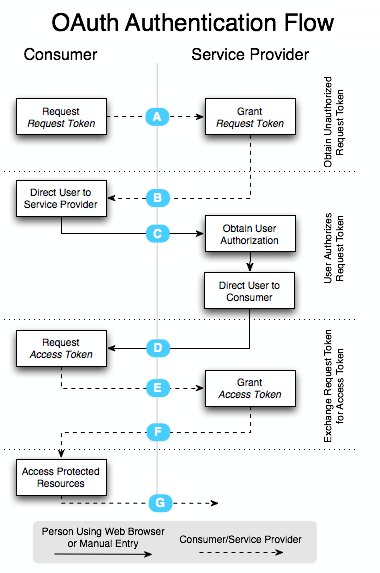
\includegraphics{figures/oauth-diagram.png}
\caption{Fragmento del diagrama de flujo de autentificación de OAuth
\label{figures:oauth}}
\end{figure}

Como puede apreciarse, implementar el protocolo OAuth manualmente
resulta algo tedioso. Son bastantes los casos que deben considerarse y
atenerse al protocolo podría tomar tiempo. Afortunadamente, existen
diferentes librerías que permiten implementar este sistema de
autentificación en muy poco tiempo. La librería Omniauth\footnote{Url!}
provee mecanismos de autentificación mediante OAuth y OpenID para
diferentes proveedores (desde GitHub hasta Google). Junto con la
librería omniauth-github, es posible implementar autentificación en muy
poco tiempo.

El primer paso es crear una ``aplicación'' en el portal de
desarrolladores de GitHub. Con esto, el proveedor entrega dos
identificadores que permiten inicializar comunicaciones con ellos y
autentificar a usuarios. En la Figura \ref{figures:oauth-create} se
puede ver el proceso de creación de aplicaciones, y en la Figura
\ref{figures:oauth-app} pueden verse ambos identificadores. Es
simplemente entregar un nombre, una URL principal (que permite a GitHub
asegurarse que las peticiones vienen del servidor que corresponde) y una
URL a la cual redirigir al usuario (que puede sobreescribirse en cada
petición).

\begin{figure}[htbp]
\centering
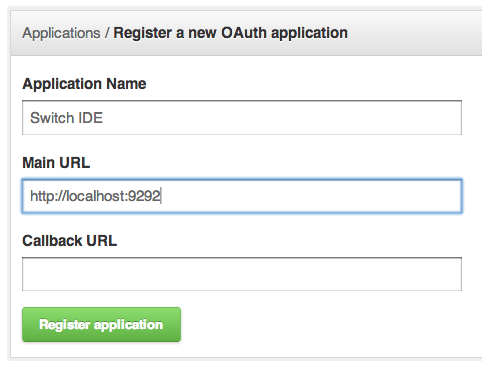
\includegraphics{figures/oauth-create.png}
\caption{Proceso de creado de aplicaciones en GitHub
\label{figures:oauth-create}}
\end{figure}

\begin{figure}[htbp]
\centering
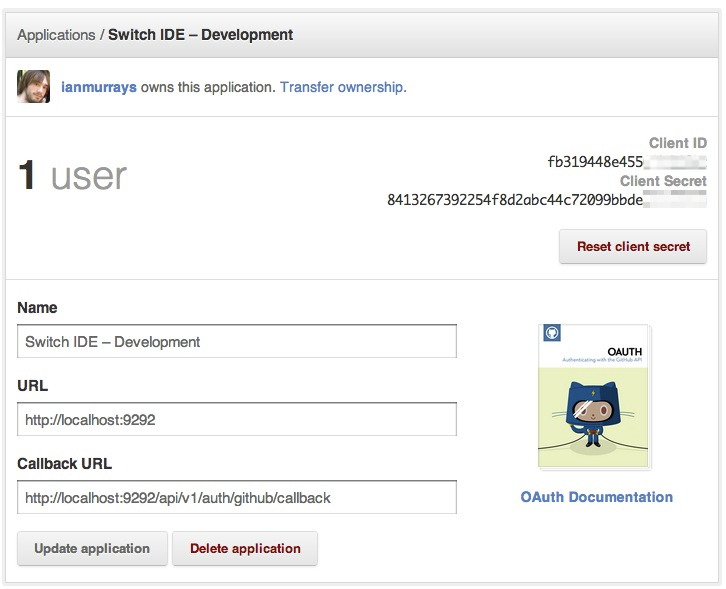
\includegraphics{figures/oauth-app.png}
\caption{Acá pueden apreciarse ambos identificadores que entrega GitHub
\label{figures:oauth-app}}
\end{figure}

\paragraph{Creación de Proyectos}

La creación de un proyecto nuevo es relativamente simple. Consiste en
crear un nuevo proyecto en la base de datos con el nombre que provee el
usuario, y luego crear el proyecto mismo utilizando Brunch.

Al crear un proyecto nuevo, el modelo guarda en la base de datos una
nueva entrada que está asociada al usuario que hace la llamada a la API.
Guarda un nombre para el proyecto, la ruta en la que fue guardado el
esqueleto y un puerto único. Antes de guardar la entrada en la base de
datos, un ``callback'' es gatillado en el mismo modelo (en Ruby) que
ejecuta el comando que crea la carpeta para el proyecto, como se detalla
a continuación:

\begin{Shaded}
\begin{Highlighting}[]
\KeywordTok{def} \NormalTok{create_project}
  \CommentTok{# Create a random path and the project}
  \DecValTok{self}\NormalTok{.path = }\StringTok{"}\OtherTok{#\{}\DecValTok{self}\NormalTok{.name}\OtherTok{\}}\StringTok{-}\OtherTok{#\{}\DataTypeTok{SecureRandom}\NormalTok{.hex(}\DecValTok{10}\NormalTok{)}\OtherTok{\}}\StringTok{"}
  \NormalTok{system }\StringTok{"brunch new }\OtherTok{#\{}\DecValTok{self}\NormalTok{.full_path}\OtherTok{\}}\StringTok{ \textbackslash{}}
\StringTok{          -s git://github.com/ianmurrays/brunch-crumbs.git"}
\KeywordTok{end}
\end{Highlighting}
\end{Shaded}

Se crea un sufijo aleatorio para evitar colisiones con proyectos que
tengan el mismo nombre, y se llama a un comando de sistema para crear el
esqueleto. Esta implementación no es perfecta, dado que podría darse el
caso de que \texttt{SecureRandom.hex(10)} arroje una cadena aleatoria
idéntica a alguna anterior. Para efectos del desarrollo del presente
trabajo, se decidió no darle demasiada importancia a este defecto, dado
que las probabilidades de que ello ocurra son demasiado bajas.

Después de que finalice este comando, se llama a un segundo ``callback''
que crea el número de puerto único para esta aplicación:

\begin{Shaded}
\begin{Highlighting}[]
\KeywordTok{def} \NormalTok{randomize_port}
  \KeywordTok{begin}
    \DecValTok{self}\NormalTok{.port = }\DecValTok{8000} \NormalTok{+ rand(}\DecValTok{2000}\NormalTok{)}
  \KeywordTok{end} \KeywordTok{until} \DataTypeTok{Project}\NormalTok{.where(port: }\DecValTok{self}\NormalTok{.port).count == }\DecValTok{0}
\KeywordTok{end}
\end{Highlighting}
\end{Shaded}

Básicamente asigna un puerto entre 8000 y 10000 aleatorio (y único) a
cada proyecto. De esta forma, si se están editando dos proyectos
simultáneamente, pueden levantarse dos instancias para hacer pruebas sin
colisionar. Esta implementación, si bien es suficiente para el
desarrollo de la herramienta y para este trabajo, no sería una
implementación ideal en producción, dado que alguno de esos puertos
podría estar siendo ocupado por algún servicio en el sistema. En una
futura implementación podría agregarse algún mecanismo que verifique la
disponibilidad del puerto al momento de asignarlo, o bien, verifique y
asigne puertos cada vez que se ensamble y corra el proyecto.

\paragraph{Manipulación de Archivos}

La manipulación de archivos se hace directamente sobre ellos usando
librerías estándar de Ruby. Sólo se discutirán algunas de las
implementaciones presentes en el backend.

Para listar los archivos presentes en una determinada ruta, se utilizó
la siguiente implementación:

\begin{Shaded}
\begin{Highlighting}[]
\KeywordTok{def} \NormalTok{files_in(folder = }\StringTok{""}\NormalTok{)}
  \CommentTok{# Remove leading and trailing slashes}
  \NormalTok{folder.gsub! }\OtherTok{/^\textbackslash{}//}\NormalTok{, }\StringTok{""}
  \NormalTok{folder.gsub! }\OtherTok{/\textbackslash{}/$/}\NormalTok{, }\StringTok{""}

  \NormalTok{files = }\DataTypeTok{Dir}\NormalTok{[}\StringTok{"}\OtherTok{#\{}\DecValTok{self}\NormalTok{.full_path}\OtherTok{\}}\StringTok{/}\OtherTok{#\{}\NormalTok{folder}\OtherTok{\}}\StringTok{/*"}\NormalTok{].collect }\KeywordTok{do} \NormalTok{\textbar{}entry\textbar{}}
    \KeywordTok{next} \KeywordTok{if}\OtherTok{ %w\{}\StringTok{server.js node_modules}\OtherTok{\}}\NormalTok{.include? }\DataTypeTok{File}\NormalTok{.basename(entry)}
    \DecValTok{self}\NormalTok{.file_to_hash entry, folder}
  \KeywordTok{end}
\KeywordTok{end}
\end{Highlighting}
\end{Shaded}

El método lista todos los archivos presentes en la ruta especificada. De
no especificarse, lista los archivos en la raíz del proyecto. Primero se
eliminan las barras (\texttt{/}) al principio y final de la ruta que se
especifique, y luego se recorre el directorio usando la clase
Dir\footnote{Http://ruby-doc.org/core-1.9.3/Dir.html.}. La llamada a
\texttt{Dir{[}"/ruta/a/directorio"{]}} retorna un array que se recorre
utilizando \texttt{collect}. El método \texttt{collect} en los arreglos
genera un nuevo arreglo con los elementos que retorne el bloque que se
le pase. \texttt{collect} pasa cada elemento del arreglo original al
bloque como argumento para su manipulación. Por ejemplo, si el siguiente
fragmento de código retorna un nuevo arreglo con sus elementos elevados
al cuadrado:

\begin{Shaded}
\begin{Highlighting}[]
\NormalTok{[}\DecValTok{1}\NormalTok{,}\DecValTok{2}\NormalTok{,}\DecValTok{3}\NormalTok{,}\DecValTok{4}\NormalTok{,}\DecValTok{5}\NormalTok{].collect }\KeywordTok{do} \NormalTok{\textbar{}num\textbar{}}
  \NormalTok{num * num}
\KeywordTok{end}

\CommentTok{# => [1,4,9,16,25]}
\end{Highlighting}
\end{Shaded}

Por lo tanto, la variable \texttt{files} en la implementación de
\texttt{files\_in} contendrá la representación en un Hash\footnote{Http://www.ruby-doc.org/core-1.9.3/Hash.html.}
(básicamente un diccionario) de cada archivo (o directorio). Además, se
excluirán el directorio \texttt{node\_modules} y el archivo
\texttt{server.js} del listado, dado que son un directorio y un archivo
que no deben ser manipulados por el desarrollador.

La implementación del método \texttt{file\_to\_hash} es relativamente
simple, y genera un diccionario con el nombre, padre y tipo de archivo
para la ruta que se le pase como parámetro:

\begin{Shaded}
\begin{Highlighting}[]
\KeywordTok{def} \NormalTok{file_to_hash(file, folder)}
  \NormalTok{\{}
    \StringTok{:name} \NormalTok{=> }\DataTypeTok{File}\NormalTok{.basename(file),}
    \StringTok{:parent} \NormalTok{=> folder,}
    \StringTok{:type} \NormalTok{=> }\KeywordTok{if} \DataTypeTok{File}\NormalTok{.directory?(file)}
      \StringTok{:directory}
    \KeywordTok{else}
      \StringTok{:file}
    \KeywordTok{end}
  \NormalTok{\}}
\KeywordTok{end}
\end{Highlighting}
\end{Shaded}

Para obtener y actualizar el contenido de archivos se utilizó una
implementación relativamente simple:

\begin{Shaded}
\begin{Highlighting}[]
\KeywordTok{def} \NormalTok{file_content(path)}
  \KeywordTok{if} \DataTypeTok{FileTest}\NormalTok{.exists? }\DecValTok{self}\NormalTok{.full_path(path) \textbackslash{}}
     \KeywordTok{and}\NormalTok{ ! }\DataTypeTok{File}\NormalTok{.directory? }\DecValTok{self}\NormalTok{.full_path(path)}
    \NormalTok{\{}
      \StringTok{:content} \NormalTok{=> }\DataTypeTok{File}\NormalTok{.read(}\DecValTok{self}\NormalTok{.full_path(path))}
    \NormalTok{\}}
  \KeywordTok{end}
\KeywordTok{end}
\end{Highlighting}
\end{Shaded}

Básicamente, se verifica que el archivo indicado exista y que no sea un
directorio, y se retorna un Hash indicando el contenido del archivo. Se
decidió retornar un Hash pues facilita su lectura en el frontend,
retornando un objeto JSON en vez del contenido directamente.

Para la escritura de archivos se utilizó una implementación similar:

\begin{Shaded}
\begin{Highlighting}[]
\KeywordTok{def} \NormalTok{update_file(path, content)}
  \KeywordTok{if} \DataTypeTok{FileTest}\NormalTok{.exists? }\DecValTok{self}\NormalTok{.full_path(path) \textbackslash{}}
     \KeywordTok{and}\NormalTok{ ! }\DataTypeTok{File}\NormalTok{.directory? }\DecValTok{self}\NormalTok{.full_path(path)}
    \DataTypeTok{File}\NormalTok{.open(}\DecValTok{self}\NormalTok{.full_path(path), }\StringTok{'w'}\NormalTok{) }\KeywordTok{do} \NormalTok{\textbar{}file\textbar{}}
      \NormalTok{file.write content}
    \KeywordTok{end}
  \KeywordTok{end}
\KeywordTok{end}
\end{Highlighting}
\end{Shaded}

Se realiza la misma verificación que al momento de obtener el contenido.
Si el archivo existe y no es una carpeta, se reemplaza todo el contenido
directamente.

El renombrado de archivos y carpetas se realiza con el siguiente método:

\begin{Shaded}
\begin{Highlighting}[]
\KeywordTok{def} \NormalTok{rename_file(path, new_path)}
  \KeywordTok{if} \DataTypeTok{FileTest}\NormalTok{.exists? }\DecValTok{self}\NormalTok{.full_path(path)}
    \DataTypeTok{File}\NormalTok{.rename }\DecValTok{self}\NormalTok{.full_path(path), }\DecValTok{self}\NormalTok{.full_path(new_path)}
  \KeywordTok{end}

  \NormalTok{directory = }\DataTypeTok{File}\NormalTok{.split(new_path).first}

  \DecValTok{self}\NormalTok{.file_to_hash }\DecValTok{self}\NormalTok{.full_path(new_path), directory}
\KeywordTok{end}
\end{Highlighting}
\end{Shaded}

Se le pasan la ruta actual y la ruta nueva del archivo, y se devuelve la
nueva representación de éste para actualizar el modelo en el frontend.
La llamada a \texttt{File.rename} permite no sólo renombrar el archivo o
directorio, sino que además permite cambiar su ruta.

\paragraph{Ensamblado y Servidor de Pruebas}

Para realizar el ensamblado se utiliza Brunch. De manera muy similar a
la creación de proyectos, es necesario ejecutar un comando de terminal
desde Ruby. La diferencia con la creación, es que acá se necesita leer
la salida del comando de manera de detectar si el ensamblado fue exitoso
o no. Para esto, se utiliza un comando distinto de \texttt{system} como
se vio antes.

\begin{Shaded}
\begin{Highlighting}[]
\KeywordTok{def} \NormalTok{build_project}
  \NormalTok{output, result = ::}\DataTypeTok{Open3}\NormalTok{.capture2e }\StringTok{"cd }\OtherTok{#\{}\DecValTok{self}\NormalTok{.full_path}\OtherTok{\}}\StringTok{ && brunch build"}

  \NormalTok{\{}
    \StringTok{:output} \NormalTok{=> output,}
    \StringTok{:result} \NormalTok{=> (output =~ }\OtherTok{/error/} \NormalTok{\textbar{}\textbar{} ! (output =~ }\OtherTok{/compiled/}\NormalTok{))}
  \NormalTok{\}}
\KeywordTok{end}
\end{Highlighting}
\end{Shaded}

La librería Open3\footnote{Http://www.ruby-doc.org/stdlib-1.9.3/libdoc/open3/rdoc/Open3.html.}
ejecutar comandos en el terminal con mayor flexibilidad. Dentro de los
comandos que provee está \texttt{capture2e}, que devuelve el output de
\texttt{stdout}y \texttt{stderr} combinados. Esto es útil en esta
situación dado que el ensamblado puede ser exitoso como no. De esta
forma, se ejecuta el comando \texttt{brunch build}, y se revisa su
output. Si éste contiene ``error'' o no contiene ``compiled'', significa
que ocurrió algún error, y el output se envía al frontend para que sea
mostrado.

Para ejecutar el servidor, se utiliza un acercamiento similar:

\begin{Shaded}
\begin{Highlighting}[]
\KeywordTok{def} \NormalTok{run_project}
  \NormalTok{output, result = ::}\DataTypeTok{Open3}\NormalTok{.capture2e }\StringTok{"cd }\OtherTok{#\{}\DecValTok{self}\NormalTok{.full_path}\OtherTok{\}}\StringTok{ \textbackslash{}}
\StringTok{                   && forever stop server.js }\OtherTok{#\{}\DecValTok{self}\NormalTok{.port}\OtherTok{\}}\StringTok{ \textbackslash{}}
\StringTok{                   && forever start server.js }\OtherTok{#\{}\DecValTok{self}\NormalTok{.port}\OtherTok{\}}\StringTok{"}

  \NormalTok{\{}
    \StringTok{:output} \NormalTok{=> output,}
    \StringTok{:url} \NormalTok{=> }\StringTok{"}\OtherTok{#\{}\DataTypeTok{Api}\NormalTok{::}\DataTypeTok{V1}\NormalTok{::}\DataTypeTok{App}\NormalTok{.settings.run_url}\OtherTok{\}}\StringTok{:}\OtherTok{#\{}\DecValTok{self}\NormalTok{.port}\OtherTok{\}}\StringTok{"}\NormalTok{,}
    \StringTok{:result} \NormalTok{=> !(output =~ }\OtherTok{/Forever processing file/}\NormalTok{)}
  \NormalTok{\}}
\KeywordTok{end}
\end{Highlighting}
\end{Shaded}

Utilizando un programa llamado ``forever''\footnote{Https://github.com/nodejitsu/forever.},
se ejecuta un script que ya se mencionó anteriormente (que además viene
con el esqueleto utilizado por brunch al crear el proyecto). Este script
levanta un servidor estático en el puerto que se especifique, y si la
ejecución fue exitosa se retorna la información necesaria al frontend.

\subsubsection{Agregado de Funcionalidad al Prototipo del Frontend}

\paragraph{Selector de Proyectos}

Se comenzó por implementar el selector de proyectos. Para esto fue
necesario implementar el modelo y colección de proyectos. En esta etapa
fueron implementados de la forma más simple posible. Básicamente, se
crearon como dos clases que extienden a \texttt{Backbone.Model} y
\texttt{Backbone.Collection} respectivamente. Dado que Backbone está
diseñado para interactuar con APIs REST, no fue necesario configurar más
que la URL del backend y especificar que la colección corresponde a una
colección de Proyectos.

\textbf{\emph{PONER EJEMPLOS DE CÓDIGO ACÁ}}

Luego de configurar el modelo y la colección, se agregó una ruta al
enrutador de Backbone. El enrutador lee la URL del navegador e
interpreta qué método llamar del enrutador. La idea es que se
especifiquen las URL necesarias para la navegación de la aplicación. En
el caso de esta solución, sólo existirán dos rutas principalmente. La
primera será la ruta base, donde se cargará el selector de proyectos del
cual se habla, y la segunda será la que tendrá cada proyecto. Por lo
tanto, se configuró la URL base, y, en el método que es llamado, se
inicializa la colección de proyectos.

\begin{Shaded}
\begin{Highlighting}[]
\NormalTok{routes}\KeywordTok{:}
  \StringTok{''}\KeywordTok{:} \StringTok{'index'}

\NormalTok{index}\KeywordTok{:} \FunctionTok{->}
  \CommentTok{# We load projects and show them on a modal window}
  \NormalTok{projects }\KeywordTok{=} \KeywordTok{new} \DataTypeTok{Projects}\KeywordTok{()}
  
  \NormalTok{projectsView }\KeywordTok{=} \KeywordTok{new} \DataTypeTok{ProjectsView}\KeywordTok{(}\NormalTok{collection}\KeywordTok{:} \NormalTok{projects}\KeywordTok{)}
  \NormalTok{$}\KeywordTok{(}\StringTok{'body'}\KeywordTok{).}\NormalTok{append projectsView}\KeywordTok{.}\NormalTok{render}\KeywordTok{().}\NormalTok{el}
  \NormalTok{$}\KeywordTok{(}\StringTok{"#}\CharTok{#\{}\NormalTok{projectsView.id}\CharTok{\}}\StringTok{"}\KeywordTok{).}\NormalTok{modal}
    \NormalTok{backdrop}\KeywordTok{:} \StringTok{'static'}
    \NormalTok{keyboard}\KeywordTok{:} \OtherTok{false}

  \NormalTok{projects}\KeywordTok{.}\NormalTok{fetch}\KeywordTok{()}
\end{Highlighting}
\end{Shaded}

En el fragmento de código anterior puede verse el método \texttt{index}
que es llamado en este punto. Luego, la colección es pasada a una vista.
Las vistas, como se explicó antes, son las encargadas de presentar datos
al usuario (por medio de templates). Esta vista, básicamente, presenta
una lista de proyectos y un formulario para crear uno nuevo (esta última
funcionalidad se creará en la segunda etapa), como puede apreciarse en
la Figura \ref{figures:projects-view}.

\begin{figure}[htbp]
\centering
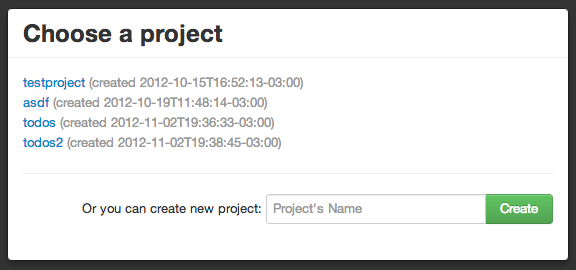
\includegraphics{figures/projects-view.png}
\caption{La ventana modal de selección de proyectos.
\label{figures:projects-view}}
\end{figure}

Al usuario hacer click en un proyecto existente, se llama a la segunda
ruta en el enrutador:

\begin{Shaded}
\begin{Highlighting}[]
\NormalTok{routes}\KeywordTok{:}
  \StringTok{''}\KeywordTok{:} \StringTok{'index'}
  \StringTok{'projects/:id'}\KeywordTok{:} \StringTok{'project'}

\NormalTok{index}\KeywordTok{:} \FunctionTok{->}
  \CommentTok{# Omitido por brevedad.}

\NormalTok{project}\KeywordTok{:} \FunctionTok{(id) ->}
  \NormalTok{app}\KeywordTok{.}\NormalTok{project }\KeywordTok{=} \KeywordTok{new} \DataTypeTok{Project}\KeywordTok{(}\NormalTok{id}\KeywordTok{:} \NormalTok{id}\KeywordTok{)}
  \NormalTok{app}\KeywordTok{.}\NormalTok{project}\KeywordTok{.}\NormalTok{fetch}
    \NormalTok{success}\KeywordTok{:} \FunctionTok{=>}
      \NormalTok{app}\KeywordTok{.}\NormalTok{filebrowser}\KeywordTok{.}\NormalTok{setModel app}\KeywordTok{.}\NormalTok{project}
      \NormalTok{Backbone}\KeywordTok{.}\NormalTok{Mediator}\KeywordTok{.}\NormalTok{pub }\StringTok{'status:set'}\KeywordTok{,} \StringTok{"Project Loaded"}

  \NormalTok{Backbone}\KeywordTok{.}\NormalTok{Mediator}\KeywordTok{.}\NormalTok{pub }\StringTok{'modal:hide'}
\end{Highlighting}
\end{Shaded}

Esta ruta, toma el identificador de proyecto de la url (que tienen un
formato estilo \texttt{proyects/IDENTIFICADOR}) e instancia un proyecto
usando ese identificador. Una vez que se haya obtenido toda su
información desde el servidor, se le asigna el modelo a la aplicación
(de manera que su instancia quede compartida) y se inicializa el visor
de archivos (que es una vista) con éste.

El visor de archivos toma el modelo de proyecto y ``pide'' su carpeta
raíz. El modelo hace una petición al backend, y éste contesta con una
representación de cada archivo (o carpeta) del directorio raíz. La
respuesta a esta llamada se presentó en la Sección
\ref{section:create-services}.

El visor de archivos, instancia una vista de archivo por cada uno de los
documentos que responde el backend. La vista de archivo se encarga de
mostrar el nombre y tipo de archivo, y permitir al usuario clickearlo
para abrirlo o ver su contenido. En caso de que el archivo se trate de
un directorio, la vista de archivo se encarga de mostrar sus contenidos.
Esta parte resultó ser un poco complicada de implementar, dado que lo
que se necesita es básicamente mostrar el mismo tipo de vista que la
raíz del proyecto pero para un subproyecto. Lo que se hizo en este caso
es lo siguiente: cuando el usuario hace click en un directorio, se
instancia una colección de archivos con la ruta a ese directorio. Se
hace una petición al servidor para que entregue la lista de archivos en
esa carpeta y se instancian vistas de archivo para cada uno,
embebiéndolas en la misma vista del directorio que se acaba de clickear.
En la Figura \ref{figure:file-browser} se puede apreciar el concepto. La
carpeta \texttt{app} es una vista de archivo, y contiene todos los
archivos y carpetas dentro de su recuadro. Lo mismo pasa con el
directorio \texttt{models}.

\begin{figure}[htbp]
\centering
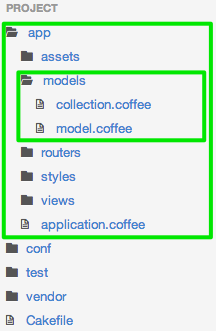
\includegraphics{figures/file-browser.png}
\caption{El visor de archivos: cada vista de directorio contiene más
vistas de archivos de ser necesarias. \label{figure:file-browser}}
\end{figure}

En caso de que el usuario haga click en un archivo, se le pasa la
instancia del modelo al editor de código, el cual indica al modelo que
debe pedir el contenido del archivo al servidor para mostrarlo. El
editor de código es simplemente una librería llamada CodeMirror que
permite al usuario editar el contenido de los archivos. El editor de
código se encarga además de indicarle al modelo del archivo que guarde
su contenido en el backend si el usuario lo solicita.

\textbf{\emph{EXPLICAR MÁS DE LO ANTERIOR}}

Para esta etapa de la construcción, se incluyó además la posibilidad de
ensamblar y ejecutar el proyecto. Para esto, se agregaron métodos en el
modelo de proyectos que hace llamadas al backend para ensamblar y
ejectuar el servidor de pruebas. El evento es manejado por la barra de
navegación, que incluye varios elementos de menú que por esta etapa se
mantuvieron inactivos. A la derecha de la barra de navegación se
encuentra un botón que permite ensamblar y ejecutar el proyecto con un
sólo click, y otros dos que permiten ejecutarlo y ensamblarlo por
separado.

En esta etapa se agregaron además atajos de teclado. Para esto se
utilizó una librería Javascript llamada Mousetrap\footnote{Link!}. Esta
librería permite configurar muy fácilmente atajos de teclado con una
gran flexibilidad en términos de combinaciones de teclas. Por ejemplo,
si se quisiera agregar un atajo de teclado para guardar el archivo
actual, se puede hacer lo siguiente:

\textbf{\emph{CORROBORAR ESTO}}

\begin{Shaded}
\begin{Highlighting}[]
\NormalTok{Mousetrap}\KeywordTok{.}\NormalTok{bind }\KeywordTok{[}\StringTok{"ctrl+s"}\KeywordTok{,} \StringTok{"command+s"}\KeywordTok{],} \FunctionTok{->}
  \CommentTok{# Guardar el archivo}
\end{Highlighting}
\end{Shaded}

Esto permite que el usuario use la combinación ``CTRL+S'' o bien, en
computadores Mac, ``COMMAND+S''. Es posible agregar atajos de teclado
más complejos, como ``CTRL+ALT+S'' o ``CTRL+SHITF+S'', etc. Incluso, es
posible saber si el usuario está manteniendo presionada alguna tecla.
Por ejemplo, si se quiere saber si el usuario está manteniendo
presionada la tecla ``SHIFT'', se puede hacer de la siguiente forma:

\textbf{\emph{PONER EXTRACTO DE CÓDIGO ACA}}

Utilizando esta librería, se agregaron varios atajos de teclado en esta
etapa. Entre ellos:

\begin{itemize}
\item
  Guardar archivo actual: \texttt{CTRL+S}
\item
  Cerrar el archivo actual: \texttt{CTRL+W}
\item
  Ejecutar el proyecto: \texttt{CTRL+R}
\item
  Cambiar entre archivos abiertos: \texttt{CTRL+NUMERO}
\end{itemize}

Este último atajo mencionado permite al usuario cambiar entre los
archivos que están abiertos en la lista de la derecha, sin tener que
mover sus manos del teclado básicamente. La mayoría de los editores de
código permiten cambiar rápidamente entre los archivos abiertos de esta
manera.

La mayoría de los atajos de teclado son interpretados por el navegador.
El atajo para guardar, para cambiar entre archivos abiertos, todos ellos
son atajos que el navegador utiliza internamente. Para evitar que el
navegador los interpretara, se utilizó el siguiente método:

\begin{Shaded}
\begin{Highlighting}[]
\NormalTok{Moustrap}\KeywordTok{.}\NormalTok{bind }\KeywordTok{[}\StringTok{"ctrl+s"}\KeywordTok{],} \FunctionTok{(event) ->}
  \NormalTok{event}\KeywordTok{.}\NormalTok{prevendDefault}\KeywordTok{()}
  
  \CommentTok{# Guardar el archivo}
\end{Highlighting}
\end{Shaded}

Cada ``evento'' que es generado en Javascript, normalmente es pasado a
los callbacks. En este caso, es posible llamar al método
\texttt{preventDefault()} del evento, lo que indica al navegador que no
realice la acción por defecto que debería. Si no se llamara a este
método, el archivo de todas formas se guardaría, pues el evento se está
llamando de todas formas, pero el navegador también mostraría la ventana
de ``Guardar Página'' que por defecto se mostraría en cualquier otro
caso, y eso no es lo que se quiere en una aplicación web de este estilo.

\subsection{Segunda Etapa de Construcción}

La segunda etapa de construccón del proyecto se dedicó principalmente a
la implementación del editor de templates. Dado que esta es la parte más
importante del proyecto se dedicó una etapa completa a ella.

El editor se diseñó de manera que en el centro se tuviera una vista en
vivo de lo que se estaba construyendo, mientras que a la derecha se
listaran todos los componentes disponibles para agregar al template.
Dado que los templates son básicamente HTML, es el navegador el que se
encarga de mostrar cómo se vería finalmente. Por esto, lo que se hizo
fue agregar elementos a la lista de componentes de manera que al
arrastrarlos hacia el centro (el editor), simplemente se agregue su
representación en HTML y el navegador se encargaría de mostrar su
``vista previa''.

Entonces, en la lista de componentes se decidió agregar botones, tablas,
formularios, campos de texto, entre otros, y dentro de ellos (en código,
no visible para el usuario) agregar un fragmento de HTML que se
agregaría al template. Entonces, utilizando jQuery UI\footnote{Definir
  esto!}, cada componente se convierte en un elemento arrastrable. Con
jQuery UI, se necesita convertir elementos en ``arrastrables'' y además,
crear elementos en donde ``soltar'' lo que el usuario está arrastrando.
En este sentido, y, en un primer intento, se convierten todos los
elementos en la vista previa en ``soltables''.

\begin{Shaded}
\begin{Highlighting}[]
\CommentTok{# Con la siguiente llamada, se convierte cada elemento en el editor}
\CommentTok{# de vistas en "soltable".}
\NormalTok{@$}\KeywordTok{(}\StringTok{"*"}\KeywordTok{).}\NormalTok{droppable}\KeywordTok{()}
\end{Highlighting}
\end{Shaded}

Con este primer acercamiento, ya se podía arrastrar y soltar
componentes. El problema es que se podían arrastar componentes como
botones y otras cosas dentro de elementos HTML que no correspondía, como
imágenes, menús, etc. Para esto, se incluyeron ciertas excepciones a la
llamada anterior, como sigue:

\begin{Shaded}
\begin{Highlighting}[]
\CommentTok{# Seleccionar todos los elementos, excepto los que están en la}
\CommentTok{# llamada .not()}
\NormalTok{@$}\KeywordTok{(}\StringTok{"*"}\KeywordTok{).not(}\StringTok{'img, button, input, select, option, optgroup'}\KeywordTok{).}\NormalTok{droppable}\KeywordTok{()}
\end{Highlighting}
\end{Shaded}

Con esto, se simplificó un tanto el arrastrado de componentes, evitando
que algunos quedaran dentro de elementos que no correspondía. Ahora, se
notó que era difícil saber dónde realmente se estaba dejando el
componente que el usuario estaba arrastrando, por lo que se incluyó
retroalimentación visual al momento de arrastar, es decir, cuando el
usuario esté arrastrando el elemento, el elemento en donde ``caería'' el
componente se rodea con un borde amarillo, como muestra la Figura
\ref{asdfaksjdha}. \textbf{\emph{PONER FIGURA!}} Esto se logra usando
propiedades de jQuery UI:

\begin{Shaded}
\begin{Highlighting}[]
\NormalTok{exceptions }\KeywordTok{=} \StringTok{'img, button, input, select, option, optgroup'}
\NormalTok{@$}\KeywordTok{(}\StringTok{"*"}\KeywordTok{).not(}\NormalTok{exceptions}\KeywordTok{).}\NormalTok{droppable}
  \NormalTok{hoverClass}\KeywordTok{:} \StringTok{"hovering"} \CommentTok{# Esto agrega una clase CSS con un borde.}
\end{Highlighting}
\end{Shaded}

La propiedad \texttt{hoverClass} agrega una clase CSS al elemento donde
se estaría arrastrando el componente y la remueve al salir. Con esto se
agrega un borde que facilite al usuario saber dónde caerá el componente.

Se decidió además agregar componentes que sólo sirven si se arrastran
dentro de un formulario. En este punto, el usuario puede arrastrar estos
componentes a cualquier parte, lo que hace de su uso algo complicado.
Para solucionar esto, se implementó un sistema en el cual cada
componente tiene especificado dónde puede ser arrastrado. Por ejemplo,
los botones pueden ser arrastrados a cualquier parte:

\begin{Shaded}
\begin{Highlighting}[]
\KeywordTok{<div}\OtherTok{ class=}\StringTok{"switch-component"}\OtherTok{ data-component-type=}\StringTok{"button"}\KeywordTok{>}
  \KeywordTok{<div}\OtherTok{ class=}\StringTok{"payload"}\KeywordTok{>}
    \KeywordTok{<button}\OtherTok{ type=}\StringTok{"button"}\OtherTok{ class=}\StringTok{"btn btn-primary"}\KeywordTok{>}\NormalTok{Button}\KeywordTok{</button>}
  \KeywordTok{</div>}

  \KeywordTok{<span}\OtherTok{ class=}\StringTok{"name"}\KeywordTok{>}\NormalTok{Button}\KeywordTok{</span>}
\KeywordTok{</div>}
\end{Highlighting}
\end{Shaded}

En cambio, los elementos de un formulario sólo pueden arrastrarse a un
formulario previamente colocado. En el siguiente fragmento se puede
notar la propiedad \texttt{data-component-drop-only} que contiene una
cadena de texto con selectores CSS en dónde puede ser agregado.

\begin{Shaded}
\begin{Highlighting}[]
\KeywordTok{<div}\OtherTok{ class=}\StringTok{"switch-component"}\OtherTok{ data-component-type=}\StringTok{"label-button"} 
\OtherTok{     data-component-drop-only=}\StringTok{"form"}\KeywordTok{>}
  \KeywordTok{<div}\OtherTok{ class=}\StringTok{"payload"}\KeywordTok{>}
    \KeywordTok{<div}\OtherTok{ class=}\StringTok{"control-group"}\KeywordTok{>}
      \KeywordTok{<div}\OtherTok{ class=}\StringTok{"control-label"}\KeywordTok{><label}\OtherTok{ for=}\StringTok{"new_input"}\KeywordTok{>}\NormalTok{Label}\KeywordTok{</label></div>}
      \KeywordTok{<div}\OtherTok{ class=}\StringTok{"controls"}\KeywordTok{>}
        \KeywordTok{<input}\OtherTok{ type=}\StringTok{"text"}\OtherTok{ name=}\StringTok{"new_input"}\OtherTok{ id=}\StringTok{"new_input"}\KeywordTok{>}
      \KeywordTok{</div>}
    \KeywordTok{</div>}
  \KeywordTok{</div>}

  \KeywordTok{<span}\OtherTok{ class=}\StringTok{"name"}\KeywordTok{>}\NormalTok{Form Input}\KeywordTok{</span>}
\KeywordTok{</div>}
\end{Highlighting}
\end{Shaded}

Lo anterior, junto con el siguiente Coffeescript, permite que los
componentes puedan ser arrastrados sólo a ciertos elementos, si es que
lo especifican:

\begin{Shaded}
\begin{Highlighting}[]
\NormalTok{makeDroppable}\KeywordTok{:} \FunctionTok{(only) ->}
  \CommentTok{# Si se especificó only, entonces usarlo, de lo contrario}
  \CommentTok{# permitir cualquier elemento.}
  \KeywordTok{if} \NormalTok{only}
    \NormalTok{only }\KeywordTok{=} \StringTok{"#view_container }\CharTok{#\{}\NormalTok{only}\CharTok{\}}\StringTok{"}
  \KeywordTok{else}
    \NormalTok{only }\KeywordTok{=} \StringTok{"#view_container, #view_container *"}

  \NormalTok{@$}\KeywordTok{(}\NormalTok{only}\KeywordTok{).not(}\NormalTok{exceptions}\KeywordTok{).}\NormalTok{droppable}
    \NormalTok{hoverClass}\KeywordTok{:} \StringTok{"hovering"}
\end{Highlighting}
\end{Shaded}

Hasta ahora, el editor de templates agrega los componentes anexándolos
al final de la posición en la que el usuario las deja. Esto lo
imposibilita de agregar componentes al principio de una lista por
ejemplo. \textbf{\emph{FIGURA EXPLICANDO ESTO?}} Por lo tanto, se agrego
la posibilidad de cambiar ese comportamiento. Al momento de arrastrar un
componente, el usuario puede presionar (y mantener presionada) la tecla
\texttt{SHIFT}, de manera que al dejar un componente, éste se anexe al
principio en vez de al final, permitiendo al usuario agregar cosas al
principio de listas o formularios, por ejemplo.

Por último, para facilitar aún más el arrastrado de componentes, se
agregó una vista previa de cómo quedaría el componente que se está
arrastrando una vez que se suelte. La idea es que al estar arrastrando
un elemento, éste aparece en el editor con una ligera opacidad. Esto se
logró usando algunas llamadas de jQuery UI:

\begin{Shaded}
\begin{Highlighting}[]
\CommentTok{# ...}
\NormalTok{@$}\KeywordTok{(}\NormalTok{only}\KeywordTok{).not(}\NormalTok{exceptions}\KeywordTok{).}\NormalTok{droppable}
  \NormalTok{hoverClass}\KeywordTok{:} \StringTok{"hovering"}
  \NormalTok{greedy}\KeywordTok{:} \OtherTok{yes}
  \NormalTok{drop}\KeywordTok{:} \FunctionTok{(e, u) ->} 
    \NormalTok{self}\KeywordTok{.}\NormalTok{putComponent}\KeywordTok{(}\NormalTok{self}\KeywordTok{,} \NormalTok{$}\KeywordTok{(}\DataTypeTok{this}\KeywordTok{),} \NormalTok{u}\KeywordTok{,} \OtherTok{no}\KeywordTok{)}
  \NormalTok{over}\KeywordTok{:} \FunctionTok{(e, u) ->}
    \NormalTok{self}\KeywordTok{.}\NormalTok{putComponent}\KeywordTok{(}\NormalTok{self}\KeywordTok{,} \NormalTok{$}\KeywordTok{(}\DataTypeTok{this}\KeywordTok{),} \NormalTok{u}\KeywordTok{,} \OtherTok{yes}\KeywordTok{)}
  \NormalTok{out}\KeywordTok{:} \FunctionTok{(e, u) ->} 
    \NormalTok{self}\KeywordTok{.}\NormalTok{removeComponent}\KeywordTok{()}
\end{Highlighting}
\end{Shaded}

Con estas llamadas, al momento de que el usuario esté sobre un elemento
(``over''), literalmente se agrega el componente al editor, para luego
eliminarlo en caso de salirse (``out''), o bien dejarlo definitivamente
al soltarlo (``drop''). \textbf{\emph{FOTOO!!!}}

Por último, el editor de templates también debería permitir al usuario
editar el código directamente, en caso de que no exista algún componente
o bien se necesite agregar cierta lógica más allá de HTML. Para esto, se
utilizó el mismo editor de código que para los archivos normales. Se
agregaron dos pestañas en la parte superior del editor de templates que
permiten cambiar entre el editor visual y el código fuente (ver Figura
\ref{figure:html-editor}).

\begin{figure}[htbp]
\centering
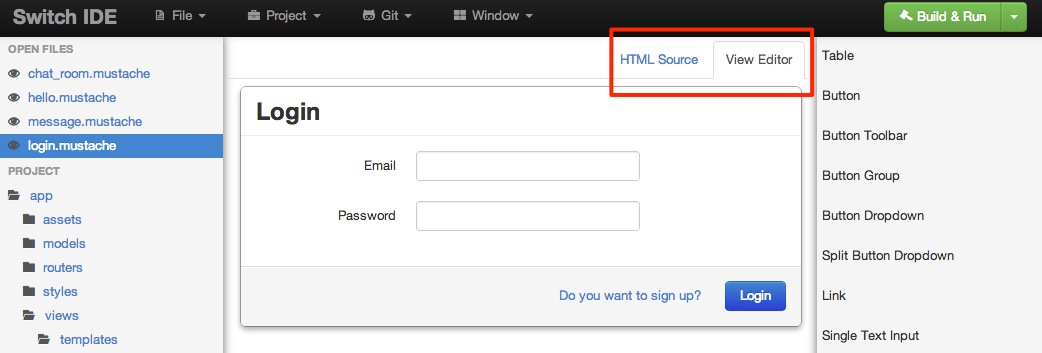
\includegraphics{figures/html-editor.png}
\caption{Estas pestañas permiten al usuario cambiar entre el modo visual
y el editor HTML \label{figure:html-editor}}
\end{figure}

\textbf{\emph{CONTENTEDITABLE!!!}}

\clearpage
\newpage

\section{Resultados}

\subsection{Producto Final}

\textbf{\emph{Explicar qué se logró, qué puede hacer}}

La herramienta que se logró en este trabajo permite desarrollar
aplicaciones web completas en un navegador. Desde la creación del
proyecto hasta la edición y ejecución de la aplicación, la solución es
una IDE completa. Se logró incluir suficiente funcionalidad como para
considerarse la solución buscada.

El componente más importante de Switch, el editor de interfaces, logra
asemejarse bastante a lo que se puede encontrar en herramientas
similares, como Xcode u otras de las mencionadas en la Sección
\ref{section:state-of-the-art}. Es un editor de uso intuitivo y con una
gran cantidad de componentes presentes en Twitter Bootstrap, lo que
permite prototipar interfaces rápida y fácilmente.

Aun cuando el editor es de fácil uso, sigue estando apuntado a usuarios
expertos (desarrolladores específicamente), y no a diseñadores u otras
personas que deseen prototipar interfaces solamente. Por esto mismo es
que el editor provee un modo de edición de HTML, para que el
desarrollador pueda realizar cambios más ``finos'' en los templates que
edite, además de tener la posibilidad de agregar más componentes que no
estarían presentes en el listado.

Además, está la posibilidad de ensamblar y probar el proyecto desde la
misma IDE. El desarrollador puede simplemente presionar ``Build \& Run''
o usar el atajo de teclado \texttt{CMD+R} (\texttt{CTRL+R} en Windows y
Linux) para que el programa ensamble y levante el servidor con el
proyecto.

\subsection{Modo de Uso de la Herramienta}

\textbf{\emph{Escribir acá un pequeño manual de cómo usar Switch}}

\subsubsection{Cómo Crear un Proyecto}

\subsubsection{Cómo Crear y Editar Archivos}

\subsubsection{Cómo Editar Vistas}

\subsubsection{Cómo Correr el Proyecto}

\subsection{Criterios de Evaluación}

La idea original de este proyecto era facilitar la creación de
interfaces y ahorrar el tiempo que se invierte en su creación. La
evaluación de la herramienta se basará en esto. Se crearán distintas
interfaces, como formularios, tablas o paneles de información, y se
medirá cuánto tiempo se requiere para crear tales interfaces usando
Switch y codificándolas directamente.

Esto permitirá medir diferentes factores que influyen. Por un lado, la
facilidad que entrega el ``arrastrar y soltar'' de componentes, y, por
otro lado, qué tanto influye la memoria del desarrollador al momento de
codificar interfaces (considerando que se usa Twitter Bootstrap).

Es importante mencionar que al momento de utilizar Switch para crear las
interfaces, también se podrá utilizar el editor de HTML (pues el poder
utilizar este editor además del editor visual es considerado una
característica), mientras que al crearlas con HTML sólo se podrá
utilizar un editor de texto, y no el editor visual.

Los ejemplos de uso que se usarán para la medición serán los siguientes:

\begin{itemize}
\item
  Un formulario de ingreso
\item
  Una tabla de usuarios
\item
  Un panel de información que consista de varias tablas
\end{itemize}

\subsection{Resultado de la Evaluación}

Para el primer caso, el formulario de ingreso se logró lo que se muestra
en la Figura \ref{figures:login-form}. El tiempo que se requirió para
construir este modelo fue de aproximadamente \textbf{3 minutos}.
Construir lo mismo manualmente tomó aproximadamente \textbf{5 minutos}.

\begin{figure}[htbp]
\centering
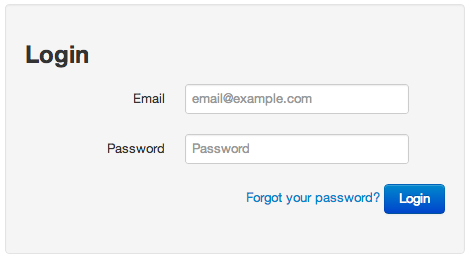
\includegraphics{figures/login-form-switch.png}
\caption{El formulario de ingreso construido usando el editor visual
\label{figures:login-form}}
\end{figure}

Para el segundo caso, se logró construir la tabla que se muestra en la
Figura \ref{figures:table-switch}. Utilizando Switch, se pudo construir
la tabla en tan sólo \textbf{2.5 minutos}, mientras que construirla sólo
con código tomó \textbf{3.5 minutos}.

\begin{figure}[htbp]
\centering
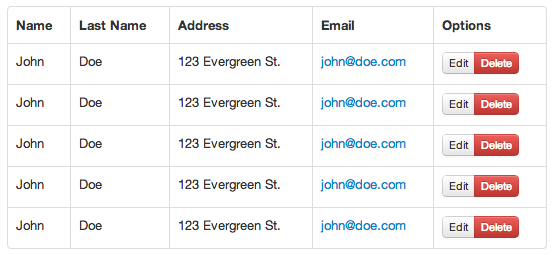
\includegraphics{figures/table-switch.png}
\caption{La tabla que se construyó con el editor
\label{figures:table-switch}}
\end{figure}

La idea del panel de información es que contenga varias tablas con
diferentes tipos de información y formularios varios. Construir el panel
usando Switch tomó aproximadamente unos \textbf{9 minutos}, mientras que
manualmente tomó \textbf{14 minutos}. El resultado se puede apreciar en
la Figura \ref{figures:dashboard}.

\begin{figure}[htbp]
\centering
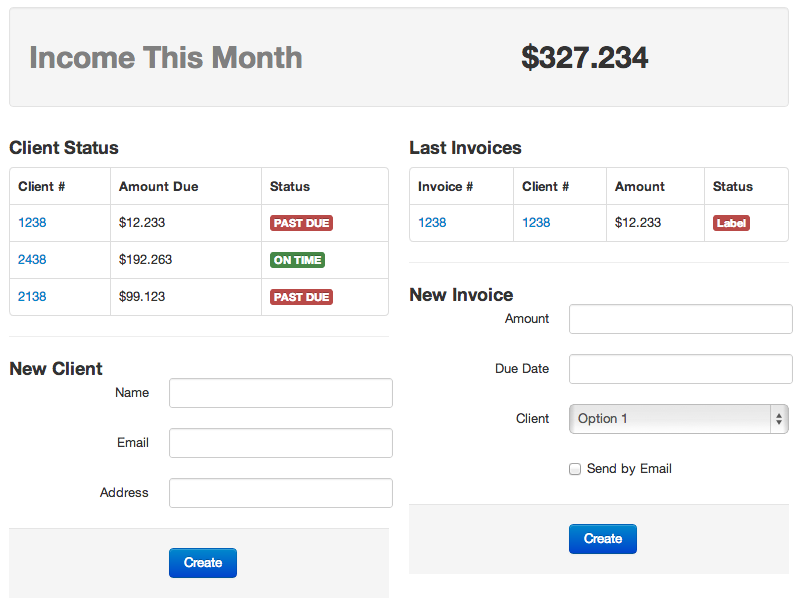
\includegraphics{figures/dashboard.png}
\caption{El panel de información o ``dashboard'' que se logró
\label{figures:dashboard}}
\end{figure}

A continuación se resumen los resultados:

\ctable[pos = H, center, botcap]{lll}
{% notes
}
{% rows
\FL
\parbox[b]{0.22\columnwidth}{\raggedright
Fruit
} & \parbox[b]{0.22\columnwidth}{\raggedright
Price
} & \parbox[b]{0.29\columnwidth}{\raggedright
Advantages
}
\ML
\parbox[t]{0.22\columnwidth}{\raggedright
Bananas
} & \parbox[t]{0.22\columnwidth}{\raggedright
\$1.34
} & \parbox[t]{0.29\columnwidth}{\raggedright
\begin{itemize}
\item
  built-in wrapper
\item
  bright color
\end{itemize}
}
\\\noalign{\medskip}
\parbox[t]{0.22\columnwidth}{\raggedright
Oranges
} & \parbox[t]{0.22\columnwidth}{\raggedright
\$2.10
} & \parbox[t]{0.29\columnwidth}{\raggedright
\begin{itemize}
\item
  cures scurvy
\item
  tasty
\end{itemize}
}
\LL
}

\ctable[pos = H, center, botcap]{lll}
{% notes
}
{% rows
\FL
\parbox[b]{0.35\columnwidth}{\raggedright
Caso de Ejemplo
} & \parbox[b]{0.28\columnwidth}{\raggedright
Tiempo con Switch
} & \parbox[b]{0.29\columnwidth}{\raggedright
Tiempo Manualmente
}
\ML
\parbox[t]{0.35\columnwidth}{\raggedright
Formulario de Ingreso
} & \parbox[t]{0.28\columnwidth}{\raggedright
3 minutos
} & \parbox[t]{0.29\columnwidth}{\raggedright
5 minutos
}
\LL
}

\textbf{\emph{PONER CONSIDERACION DE QUE IGUAL CACHO HARTO DE BOOTSTRAP
:D}}

\clearpage
\newpage

\section{Conclusiones}

A continuación se presentarán conclusiones del presente trabajo, en
respecto a la solución lograda, su efectividad, la metodología empleada,
características que no se pudieron agregar (y las respectivas razones),
y conclusiones para un trabajo futuro.

\subsection{Sobre la Solución}

La solución que se presenta en este documento permite disminuir los
tiempos de desarrollo de soluciones web, facilitando la tarea que más
tiempo consume. El prototipado y construcción de vistas en aplicaciones
de cualquier tipo siempre es la más tediosa, sobre todo en el ambiente
web donde todo debe hacerse por código. Usando Switch IDE, se facilita
gran parte de esta tarea proveyendo al desarrollador con componentes
utilizados comúnmente en el desarrollo de aplicaciones, como botones,
formularios, tablas, entre otras.

Sin embargo, posee algunas desventajas. Cada vez que se quiere probar
algún cambio realizado en el programa, hay que reensamblar el proyecto,
lo que toma tiempo. Esto, en todo caso, puede solucionarse y se discute
en la Sección \ref{section:future-work} del presente capítulo. Otra
desventaja que presenta la solución es que agregar lógica a los
templates (como se hace normalmente en desarrollo web), es difícil. Por
ejemplo, si se desea mostrar un botón sólo en caso de que alguna
variable sea verdadera en el controlador, se debe agregar código a la
vista y eso hace que el editor visual muestre este código. Soluciones a
este problema se discuten también en la Sección
\ref{section:future-work}.

\subsection{Sobre la Metodología}

El haber dividido el proceso de construcción en dos fases permitió
evaluar la efectividad de las herramientas escogidas antes de comenzar
con la programación del aspecto más importante de la solución. La
primera fase involucró la creación del backend de manera casi completa,
el prototipado de la interfaz y la creación de una base para el
desarrollo de la segunda etapa.

La división en dos fases fue acertada, y el orden del desarrollo de los
diferentes componentes fue correcto, dado que de haber prototipado el
editor de interfaces antes de comenzar con la base, se podría haber
creado (accidentalmente) un editor completamente incompatible con la
solución final. Ahora bien, el haber prototipado un editor de interfaces
antes de comenzar con el desarrollo podría haber revelado dificultades
que se podrían haber encontrado en la segunda etapa (aunque de todas
formas se sabía que era posible desarrollar algo de esa índole dado que
existían herramientas similares).

\subsection{Sobre la Elección de Herramientas}

\subsubsection{Herramientas del Backend}

Haber elegido Ruby y Sinatra para construir el backend fue una buena
decisión. Permitió crear un backend simple, liviano y mantenible en poco
tiempo.

\textbf{\emph{YA Y?}}

\subsubsection{Herramientas del Frontend}

En un principio se escogió Backbone para construir el frontend por su
simplicidad, popularidad y por ser un framework liviano. Hubo que
considerar que el autor no poseía conocimientos con ninguno de estos
frameworks inicialmente, por lo que la elección se vio sesgada hacia una
herramienta fácil de aprender y con buena documentación y soporte (o
sea, una comunidad activa).

Backbone probó ser un framework fácil de dominar y muy flexible. La
presencia de varias librerías y extensa documentación en línea permitió
dominar la herramienta en poco tiempo y crear una solución mantenible y
legible.

\subsection{Características que Faltaron}

\textbf{\emph{NO SÉ SI AGREGAR ESTO EN LA MEMORIA}}

La principal característica que se omitió fue la de poder ``unir''
elementos con acciones en el editor de vistas. Por ejemplo, al agregar
un botón, la idea sería conectarlo con el controlador de manera que al
hacer click se ejecutara una determinada acción. En Xcode es posible
presionar \texttt{CTRL} y arrastrar el componente hacia el código, y
automáticamente se genera una acción que se ejecutaría al presionar el
componente. Ver Figura \ref{figure:xcode-ctrl-drag}.

\begin{figure}[htbp]
\centering
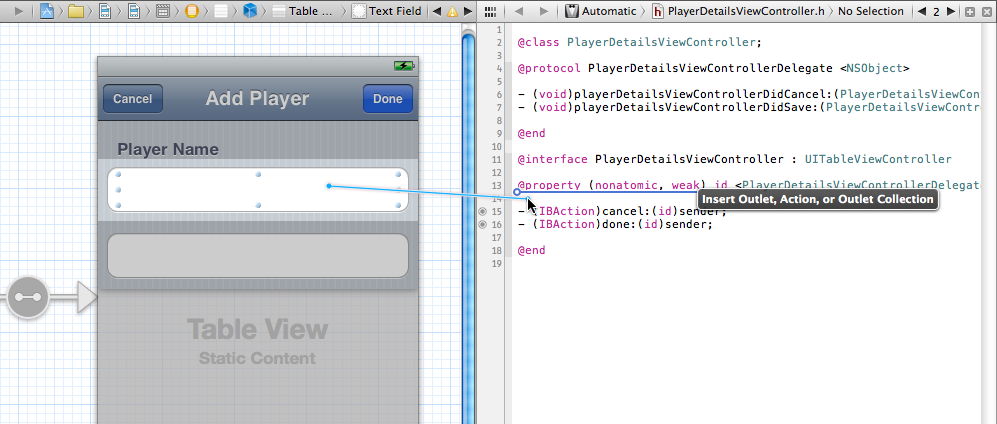
\includegraphics{figures/xcode-ctrl-drag.png}
\caption{Al presionar la tecla \texttt{CTRL} y arrastrar, es posible
crear métodos directamente. \label{figure:xcode-ctrl-drag}}
\end{figure}

Otro feature que no se agregó es el de archivar los proyectos. Archivar
significa básicamente ensamblar el proyecto y dejarlo listo para su
implementación en un servidor. La idea de esta característica es
ensamblar y comprimir el proyecto en un archivo zip para su posterior
descarga.

\subsection{Trabajo Futuro}

\label{section:future-work}

Una de las características que sería ideal agregar a una futura versión
es la de control de versiones con Git. Agregar esta característica no
sería trivial pero tampoco sería extremadamente difícil dado que existen
librerías que lo facilitarían. Agregar esta funcionalidad permitiría a
los desarrolladores mantener su código versionado y además permitiría la
colaboración, por medio de repositorios compartidos.

Agregar esta funcionalidad requeriría de interfaces que permitan al
desarrollador seleccionar archivos para agregar al repositorio, crear
nuevos ``commits'' (como se le conoce a los estados de código en
versionamiento), descargar y subir cambios a repositorios remotos y
poder (al menos) ver el historial del repositorio.

Otra característica importante que se discutió antes es la de no
necesitar ensamblar el proyecto constantemente. Brunch (el ensamblador
que se utilizó en este trabajo) permite levantar un proceso que observa
cambios en los archivos y ensambla el proyecto bajo demanda. Eso hace
que el proceso de programar y probar los cambios sea mucho más continuo
y simple. \textbf{\emph{Tal vez hablar más de esto?}}

Una adición que podría ser de importancia en proyectos con archivos
grandes sería la de no enviar el archivo completo cada vez que se
guarden cambios. Este es el comportamiento actual y, si bien no se nota
para archivos livianos, sí se sentiría al momento de guardar archivos de
100 o más líneas de código. Una posible solución sería enviar parches,
es decir, guardar en el frontend el estado en el que se encuentra el
archivo en el servidor, y, al momento de guardar cambios, enviar sólo
las diferencias de manera de minimizar la cantidad de información
enviada. De esta forma, si se tuviera un archivo con 200 líneas de
código y sólo se quisiera agregar 2 líneas con comentarios, se ahorraría
un 99\% de cantidad de datos que se transfieran.

Un cambio que no sería menor, y que está relacionado con la edición de
vistas, es la de cambiar el framework que se utiliza para el desarrollo
por una conocida como Knockback\footnote{Referencia.}. Knockback es una
combinación de dos frameworks: Backbone (la que se utiliza actualmente)
y Knockout. Knockout es conocido por ofrecer ``bindings'', es decir,
permite agregar atributos HTML a las vistas de manera que se actualicen
automáticamente, sin necesidad de escribir código dentro de ellas. Como
por ejemplo:

\begin{Shaded}
\begin{Highlighting}[]
\KeywordTok{<p>}\NormalTok{First name: }\KeywordTok{<strong}\OtherTok{ data-bind=}\StringTok{"text: firstName"}\KeywordTok{></strong></p>}
\KeywordTok{<p>}\NormalTok{Last name: }\KeywordTok{<strong}\OtherTok{ data-bind=}\StringTok{"text: lastName"}\KeywordTok{></strong></p>}
\end{Highlighting}
\end{Shaded}

El fragmento anterior une las etiquetas
\texttt{\textless{}strong\textgreater{}} con los atributos
\texttt{firstName} y \texttt{lastName} del modelo asociado. Lo ventajoso
es que es simple HTML y además las uniones son en tiempo real, lo que
significa que cualquier cambio al modelo ocurrirá en la vista sin
requerir ningún esfuerzo extra por parte del desarrollador.

Esto mejoraría la experiencia del usuario al momento de diseñar vistas
dado que no necesitaría escribir código (sólo HTML). Además, y más
importante, esto permitiría mejorar el editor de interfaces de manera de
que el usuario agregue ``bindings'' visualmente, con menús contextuales,
sin editar el código fuente de la vista.

Agregar este framework requeriría cierto esfuerzo, aunque Brunch
facilita esta tarea permitiendo crear ``esqueletos'' para proyectos con
este framework. Exportar proyectos ya existentes no sería trivial, pero
tampoco sería muy complejo, dado que Knockback simplemente combina ambos
frameworks.

\clearpage
\newpage

\section{Referencias}

{[}1{]} Steve Burbeck, ``Applications Programming in Smalltalk-80(TM):
How to use Model-View-Controller (MVC)'' Disponible:
\href{http://st-www.cs.illinois.edu/users/smarch/st-docs/mvc.html}{http://st-www.cs.illinois.edu/users/smarch/st-docs/mvc.html}.
Última Revisión: 09/07/2012.

{[}2{]} Mike Potel, ``MVP: Model-View-Presenter. The Taligent
Programming Model for C++ and Java'' Disponible:
\href{http://www.wildcrest.com/Potel/Portfolio/mvp.pdf}{http://www.wildcrest.com/Potel/Portfolio/mvp.pdf}.
Última Revisión: 09/07/2012.

{[}3{]} DocumentCloud, ``Backbone'' Disponible:
\href{http://backbonejs.org}{http://backbonejs.org}. Última Revisión:
09/07/2012.

{[}4{]} Backbone, ``Projects and Companies using Backbone'' Disponible:
\href{https://github.com/documentcloud/backbone/wiki/Projects-and-Companies-using-Backbone}{https://github.com/documentcloud/backbone/wiki/Projects-and-Companies-using-Backbone}.
Última Revisión: 09/07/2012.

{[}5{]} Cappuccino Project, ``Cappuccino Framework'' Disponible:
\href{http://www.cappuccino-project.org/}{http://www.cappuccino-project.org/}.
Última Revisión: 09/07/2012.

{[}6{]} Apple Inc., ``Xcode'' Disponible:
\href{https://developer.apple.com/xcode/}{https://developer.apple.com/xcode/}.
Última Revisión: 09/07/2012.

{[}7{]} Sencha Inc., ``Ext JS'' Disponible:
\href{http://www.sencha.com/products/extjs/}{http://www.sencha.com/products/extjs/}.
Última Revisión: 09/07/2012.

{[}8{]} Sencha Inc., ``Ext JS Releases'' Disponible:
\href{http://www.sencha.com/products/releases/}{http://www.sencha.com/products/releases/}.
Última Revisión: 09/07/2012.

{[}9{]} Sencha Inc., ``Buy Ext JS 4 Licenses and Support'' Disponible:
\href{http://www.sencha.com/store/extjs/}{http://www.sencha.com/store/extjs/}.
Última Revisión: 09/07/2012.

{[}10{]} Sencha Inc., ``Sencha Architect'' Disponible:
\href{http://www.sencha.com/products/architect/}{http://www.sencha.com/products/architect/}.
Última Revisión: 09/07/2012.

{[}11{]} Sencha Inc., ``Buy Sencha Architect'' Disponible:
\href{http://www.sencha.com/store/architect/}{http://www.sencha.com/store/architect/}.
Última Revisión: 09/07/2012.

{[}12{]} Divshot, ``Divshot'' Disponible:
\href{http://www.divshot.com}{http://www.divshot.com}. Última Revisión:
09/07/2012.

{[}13{]} Twitter, ``Twitter Bootstrap'' Disponible:
\href{http://getbootstrap.com}{http://getbootstrap.com}. Última
Revisión: 09/07/2012.

{[}14{]} Ian Hickson (editor), ``HTML5 Specification'' Disponible:
\href{http://www.w3.org/TR/2011/WD-html5-20110525/}{http://www.w3.org/TR/2011/WD-html5-20110525/}.
Última Revisión: 09/07/2012.

{[}15{]} eXo Platform SAS, ``eXo Cloud IDE'' Disponible:
\href{http://cloud-ide.com}{http://cloud-ide.com}. Última Revisión:
09/07/2012.

{[}16{]} Git Project, ``Git'' Disponible:
\href{http://git-scm.com}{http://git-scm.com}. Última Revisión:
09/07/2012.

{[}17{]} VMware Inc., ``Wavemaker'' Disponible:
\href{http://wavemaker.com}{http://wavemaker.com}. Última Revisión:
09/07/2012.

{[}18{]} Zoho Corp., ``Zoho Creator'' Disponible:
\href{http://www.zoho.com/creator/}{http://www.zoho.com/creator/}.
Última Revisión: 09/07/2012.

\end{document}
